\documentclass[12pt]{article}
\usepackage{fullpage}
\usepackage[utf8]{inputenc}
\usepackage{pict2e}
\usepackage{amsmath}
\usepackage{enumitem}
\usepackage{eurosym}
\usepackage{pict2e}
\usepackage{mathtools}
\usepackage{amssymb, amsfonts, latexsym, cancel}
\setlength{\parskip}{0.3cm}
\usepackage{graphicx}
\usepackage{fontenc}
\usepackage{slashbox}
\usepackage{setspace}
\usepackage{gensymb}
\usepackage{accents}
\usepackage{adjustbox}
\setstretch{1.5}
\usepackage{bold-extra}
\usepackage[document]{ragged2e}
\usepackage{subcaption}
\usepackage{tcolorbox}
\usepackage{xcolor, colortbl}
\usepackage{wrapfig}
\usepackage{empheq}
\usepackage{array}
\usepackage{parskip}
\usepackage{arydshln}
\graphicspath{ {images/} }
\renewcommand*\contentsname{\color{black}Índice} 
\usepackage{array, multirow, multicol}
\definecolor{lightblue}{HTML}{007AFF}
\usepackage{color}
\usepackage{etoolbox}
\usepackage{listings}
\usepackage{mdframed}
\setlength{\parindent}{0pt}
\usepackage{underscore}
\usepackage{hyperref}
\usepackage{tikz}
\usepackage{tikz-cd}
\usetikzlibrary{shapes, positioning, patterns}
\usepackage{tikz-qtree}
\usepackage{biblatex}
\usepackage{pdfpages}
\usepackage{pgfplots}
\usepackage{pgfkeys}
\addbibresource{biblatex-examples.bib}
\usepackage[a4paper, left=1.5cm, right=1.5cm, top=1cm,
bottom=1.5cm]{geometry}
\everymath{\displaystyle}
\usetikzlibrary{decorations.pathreplacing}
\usepackage{titlesec}
\usepackage{titletoc}
\usepackage{tikz-3dplot}
\usetikzlibrary{decorations.pathreplacing}
\newcommand{\Ej}{\textcolor{lightblue}{\underline{Ejemplo}}}
\setlength{\fboxrule}{1.5pt}
\renewcommand{\arraystretch}{1.35}
\setlength{\arraycolsep}{0.3cm}

% Configura el formato de las secciones utilizando titlesec
\titleformat{\section}
{\color{red}\normalfont\LARGE\bfseries}
{Tema \thesection:}
{10 pt}
{}

% Ajusta el formato de las entradas de la tabla de contenidos
\addtocontents{toc}{\protect\setcounter{tocdepth}{4}}
\addtocontents{toc}{\color{black}}

\titleformat{\subsection}
{\normalfont\Large\bfseries\color{red}}{\thesubsection)}{1em}{\color{lightblue}}

\titleformat{\subsubsection}
{\normalfont\large\bfseries\color{red}}{\thesubsubsection)}{1em}{\color{lightblue}}

\newcommand{\bboxed}[1]{\fcolorbox{lightblue}{lightblue!10}{$#1$}}

\DeclareMathOperator{\N}{\mathbb{N}}
\DeclareMathOperator{\Z}{\mathbb{Z}}
\DeclareMathOperator{\R}{\mathbb{R}}
\DeclareMathOperator{\Q}{\mathbb{Q}}
\DeclareMathOperator{\K}{\mathbb{K}}
\DeclareMathOperator{\im}{\imath}
\DeclareMathOperator{\jm}{\jmath}
\DeclareMathOperator{\col}{\mathrm{Col}}
\DeclareMathOperator{\fil}{\mathrm{Fil}}
\DeclareMathOperator{\rg}{\mathrm{rg}}
\DeclareMathOperator{\nuc}{\mathrm{nuc}}
\DeclareMathOperator{\dimf}{\mathrm{dimFil}}
\DeclareMathOperator{\dimc}{\mathrm{dimCol}}
\DeclareMathOperator{\dimn}{\mathrm{dimnuc}}
\DeclareMathOperator{\dimr}{\mathrm{dimrg}}

\newcommand{\bu}[1]{\textcolor{lightblue}{\underline{#1}}}
\newcommand{\lb}[1]{\textcolor{lightblue}{#1}}
\newcommand{\db}[1]{\textcolor{blue}{#1}}
\newcommand{\rc}[1]{\textcolor{red}{#1}}
\newcommand{\tr}{^\intercal}

\renewcommand{\CancelColor}{\color{lightblue}}

\newcommand{\dx}{\:\mathrm{d}x}
\newcommand{\dt}{\:\mathrm{d}t}
\newcommand{\dy}{\:\mathrm{d}y}
\newcommand{\dz}{\:\mathrm{d}z}
\newcommand{\dth}{\:\mathrm{d}\theta}
\newcommand{\dr}{\:\mathrm{d}\rho}
\newcommand{\du}{\:\mathrm{d}u}
\newcommand{\dv}{\:\mathrm{d}v}
\newcommand{\tozero}[1]{\cancelto{0}{#1}}
\newcommand{\lbb}[2]{\textcolor{lightblue}{\underbracket[1pt]{\textcolor{black}{#1}}_{#2}}}
\newcommand{\dbb}[2]{\textcolor{blue}{\underbracket[1pt]{\textcolor{black}{#1}}_{#2}}}
\everymath{\displaystyle}

\begin{document}
\begin{enumerate}[label=\color{red}\textbf{\arabic*)}, leftmargin=*]
	\item \lb{Determinar el dominio de definición de las siguientes funciones:}
	
	$\db{f(x)=x-\sqrt{\dfrac{x+2}{x-1}}}$
	
	Para empezar, como hay un cociente debemos evitar que el denominador sea cero \begin{center}
		$x-1=0\longrightarrow\bboxed{x=1}$ No está en el dominio
	\end{center}
	Por otro lado, tenemos una raíz cuadrado y esto implica que la de dentro, debe ser positivo o cero: $\dfrac{x+2}{x-1}\ge0$
	\begin{center}
		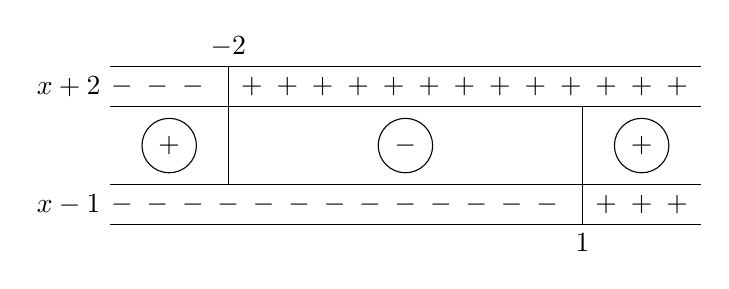
\begin{tikzpicture}[xscale=1.5]
			\draw (-3,0) -- (2,0)
			(-3,-0.5) -- (2,-0.5)
			(-3,-1.5) -- (2,-1.5)
			(-3,-2) -- (2,-2);
			\node[left] at (-3,-0.25) {$x+2$};
			\node[left] at (-3,-1.75) {$x-1$};
			\foreach \x in {-2.9, -2.6, ..., -2.1}{
			\node at (\x, -0.25) {$-$};
			}
			\foreach \x in {-2.9, -2.6, ..., 0.8}{
			\node at (\x, -1.75) {$-$};
			}
			\foreach \x in {-1.8, -1.5, ..., 2}{
			\node at (\x, -0.25) {$+$};
			}
			\foreach \x in {1.2, 1.5, ..., 2}{
			\node at (\x, -1.75) {$+$};
			}
			\draw (-2,0) node[above] {$-2$} -- (-2,-1.5) ;
			\draw (1,-0.5) -- (1,-2) node[below] {$1$} ;
			\node[circle, draw=black] at (-2.5,-1) {+};
			\node[circle, draw=black] at (1.5,-1) {+};
			\node[circle, draw=black] at (-0.5,-1) {$-$};
		\end{tikzpicture}
	\end{center}
	$\dfrac{x+2}{x-1}\ge0\longrightarrow x\in(-\infty,-2]\cup(1,+\infty)$
	
	Por lo tanto el dominio de la función es: \[ \bboxed{\dom(f)=(-\infty,-2]\cup(1,+\infty)} \]
	\item \lb{Determinar el dominio de definición de las siguientes funciones:}
	
	$\db{f(x)=\sqrt[4]{\dfrac{x}{\log(x)}}}$
	
	Como hay un cociente entonces el denominador no puede ser cero: \begin{center}
		$\log(x)=0\longrightarrow\bboxed{x=1}$ No está en el dominio
	\end{center}
	Como hay un logaritmo, lo de dentro solo puede ser positivo: \[ \bboxed{x>0} \]Como tenemos una raíz cuarta (de grado par) entonces lo de dentro no puede ser negativo:
	
	\begin{minipage}{0.4\textwidth}
		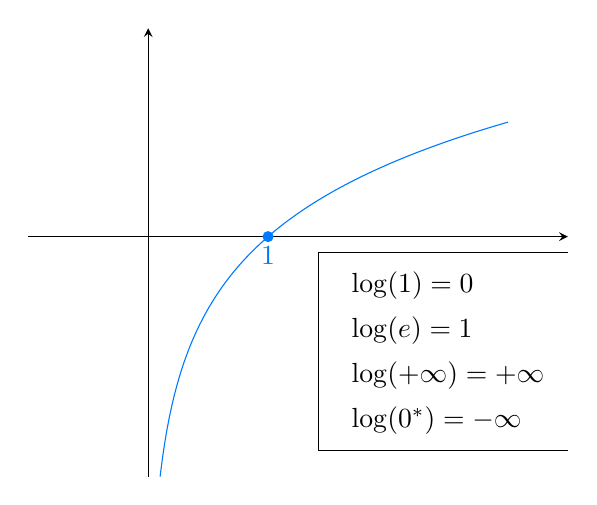
\begin{tikzpicture}
			\begin{axis}[xmin=-1, xmax=3.5, ymax=2, axis lines=center, xtick=\empty, ytick=\empty]
				\addplot[lightblue, domain=0.1:3, samples=150] {ln(x)};
				\fill[lightblue] (axis cs:1,0) circle (2pt) node[below] {$1$};
				\node[rectangle, draw=black] at (axis cs:2.5,-1.1) {$\begin{array}{l}
						\log(1)=0\\
						\log(e)=1\\
						\log(+\infty)=+\infty\\
						\log(0^*)=-\infty\\
					\end{array}$};
			\end{axis}
		\end{tikzpicture}
	\end{minipage}\qquad\begin{minipage}{0.45\textwidth}
	$\dfrac{x}{\log(x)}\ge0\longrightarrow x\in(1,+\infty)$
	\begin{center}
		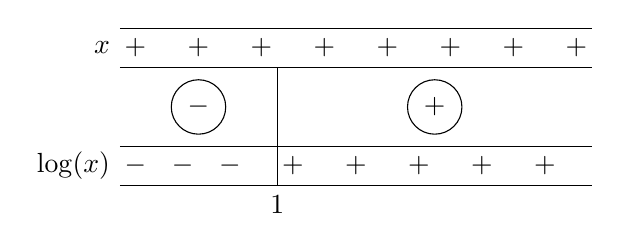
\begin{tikzpicture}[xscale=2]
			\draw (0,0) -- (3,0)
			(0,-0.5) -- (3,-0.5)
			(0,-1.5) -- (3,-1.5)
			(0,-2) -- (3,-2)
			;
			\foreach \x in {0.1, 0.5, ..., 3}{\node at (\x, -0.25) {$+$};}
			\foreach \x in {0.1, 0.4, ..., 0.8}{\node at (\x, -1.75) {$-$};}
			\foreach \x in {1.1, 1.5, ..., 3}{\node at (\x, -1.75) {$+$};}
			\draw (1,-0.5) -- (1,-2) node[below] {$1$};
			\node[circle, draw=black] at (0.5, -1) {$-$};
			\node[circle, draw=black] at (2, -1) {$+$};
			\node[left] at (0,-0.25) {$x$};
			\node[left] at (0,-1.75) {$\log(x)$};
		\end{tikzpicture}
	\end{center}
	Por lo tanto: \[ \bboxed{\dom(f)=(1,+\infty)} \]
	\end{minipage}
	\item \lb{Vamos a comprobar si la aplicación \[ \begin{aligned}
			f:&\R\longrightarrow\R\\
			&x\longmapsto f(x)=2x+1
		\end{aligned} \]es biyectiva, es decir, si es inyectiva y sobreyectiva.}
	
	\begin{minipage}{0.5\textwidth}
		Veamos si la aplicación $f(x)$ es inyectiva:
		\begin{itemize}[leftmargin=*]
			\item Sea: \[ f(x_1)=f(x_2)\longrightarrow2x_1+1=2x_2+1\longrightarrow\bboxed{x_1=x_2} \]Por lo tanto: $f(x)$ es inyectiva.
			\item Por otro lado: $\forall y\in\R\longrightarrow y=f(x)=2x+1$ 
			\begin{center}
				$2x=1-y\longrightarrow x=\dfrac{1-y}{2}$ Por lo tanto $\forall y\in\R$ existe un $x\in\R$ tal que $f(x)=y$$\longrightarrow f(x)$ es sobreyectiva.
			\end{center}
		\end{itemize}
		
	\end{minipage}\qquad\begin{minipage}{0.4\textwidth}
	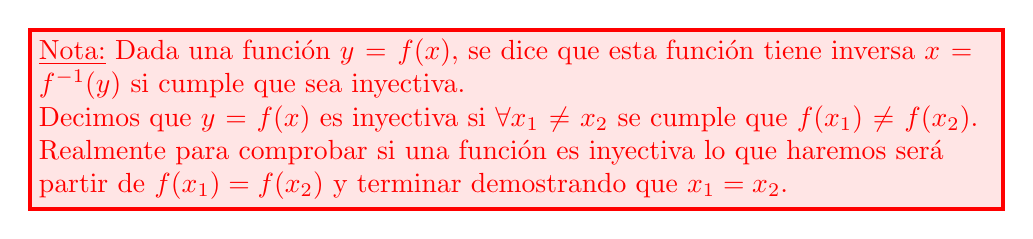
\begin{tikzpicture}
		\node[red, draw=red, fill=red!10, line width=1.5, text width=\linewidth] {\underline{Nota:} Dada una función $y=f(x)$, se dice que esta función tiene inversa $x=f^{-1}(y)$ si cumple que sea inyectiva.\\
		Decimos que $y=f(x)$ es inyectiva si $\forall x_1\neq x_2$ se cumple que $f(x_1)\neq f(x_2)$. Realmente para comprobar si una función es inyectiva lo que haremos será partir de $f(x_1)=f(x_2)$ y terminar demostrando que $x_1=x_2$.};
	\end{tikzpicture}
	\end{minipage}
	
	Entonces, como $f(x)$ es inyectiva y sobreyectiva en todo $\R$ podemos asegurar que $f(x)$ es biyectiva y por lo tanto existe su función inversa. \[ \begin{aligned}
		f^{-1}:&\R\longrightarrow\R\\
		&y\longrightarrow x=f^{-1}(y)=\dfrac{1-y}{2}
	\end{aligned} \]
	
\item \lb{Comprobar si la función $f:\R\longrightarrow\R$ con $f(x)=x^2$ tiene inversa.}

Para que tenga inversa debe ser inyectiva, y esto implica que para elementos diferentes debe tener diferentes y como: 
\begin{center}
	$\begin{rcases}
		f(1)=1\\
		f(-1)=1
	\end{rcases}$ No es inyectiva $\longrightarrow f(x)$ No tiene inversa
\end{center}
\item \lb{Dadas las siguientes funciones, averiguar en qué puntos son discontinuas y por qué.}

$\db{f(x)=\dfrac{x^2}{x-2}\text{ si }x\neq0,\, f(2)=0.}$

$f(x)=\begin{cases}
	\dfrac{x^2}{x-2} & \text{si }x\neq2\\
	0 & \text{si }x=2
\end{cases}$\\
$\forall x\neq2\:f(x)$ es continua por ser un cociente de funciones continuas con denominador distinto de cero.

Veamos ahora si es continua en $x=2$.

\begin{center}
	$\begin{rcases}
	\lim_{x\to2^-}\dfrac{x^2}{x-2}=\dfrac{4}{0^-}=-\infty\\
	\lim_{x\to2^+}\dfrac{x^2}{x-2}=\dfrac{4}{0^+}=+\infty\\
\end{rcases}$\quad\begin{minipage}{0.5\textwidth}
$f(x)$ No es continua en $x=2$, en concreto presenta en $x=2$ una discontinuidad inevitable de salto infinito. Diremos que $f(x)$ presenta en $x=2$ una asíntota vertical.
\end{minipage}\\
\begin{tikzpicture}
	\begin{axis}[xmin=-1, xtick=\empty, ytick=\empty, axis lines=center, xmax=4]
		\addplot[lightblue, line width=1.5, domain=2.1:2.2] {x^2/(x-2)};
		\addplot[lightblue, line width=1.5, domain=1.7:1.9] {x^2/(x-2)};
		\draw[lightblue] (axis cs:2,50) -- (axis cs:2,-50);
		\fill[lightblue] (axis cs:2,0) circle (2pt) node[ below right] {$2$};
	\end{axis}
\end{tikzpicture}
\end{center}
\item \lb{Determinar el dominio de definición de las siguientes funciones:}

$\db{f(x)=\dfrac{1}{\sqrt{1-e^x}}}$

Como es un cociente, debemos evitar que el denominador sea cero: \begin{center}
	$1-e^x=0\longrightarrow e^x=1\longrightarrow x=\ln(1)=0\longrightarrow\bboxed{x=0}$ No pertenece el dominio
\end{center}
Como hay una raíz cuadrada, lo de dentro no puede ser negativo: \[ 1-e^x>0\longrightarrow e^x<1\longrightarrow x<\ln(1)=0\longrightarrow\bboxed{x<0} \]
\fcolorbox{lightblue}{lightblue!10}{Por lo tanto, el $\dom(f)=(-\infty,0)$}
\item \lb{Estudiar la continuidad de la función \[ f(x)=\begin{cases}
		-xe^{x-1} & \text{si }x<0\\
		xe^{x-1} & \text{si }0\le x<1\\
		xe^{1-x} & \text{si }x\ge1
	\end{cases} \]}
$\forall x<0\longrightarrow f(x)=-xe^{x-1}$ es continua por ser un producto de funciones continuas\\
$\forall x\in(0,1)\longrightarrow f(x)=xe^{x-1}$ es continua por ser un producto de funciones continuas\\
$\forall x>1\longrightarrow f(x)=xe^{1-x}$ es continua por ser un producto de funciones continuas\\
Veamos ahora si $f(x)$ es continua en $x=0$ y $x=1$:
\begin{itemize}[label=]
	\item \underline{En $x=0$:}
	\begin{center}
		$\begin{rcases}
			\lim_{x\to0^-}(-xe^{x-1})=0\\
			\lim_{x\to0^+}(xe^{1-x})=0\\
		\end{rcases}\begin{array}{l}
		\lim_{x\to0}f(x)=0\\
		f(0)=0
		\end{array}~~$\begin{minipage}{0.5\textwidth}
		Como existe el límite de $f(x)$ en $x=0$ y coincide con $f(0)$ entonces podemos asegurar que $f(x)$ es continua en $x=0$.
		\end{minipage}
	\end{center}
	\item \underline{En $x=1$:}
	\begin{center}
		$\begin{rcases}
			\lim_{x\to1^-}xe^{x-1}=1\\
			\lim_{x\to1^+}xe^{1-x}=1
		\end{rcases}\begin{array}{l}
		\lim_{x\to1}f(x)=1\\
		f(1)=1
		\end{array}~~$\begin{minipage}{0.5\textwidth}
		Como existe el límite de $f(x)$ en $x=1$ y coincide con $f(1)$ entonces podemos asegurar que $f(x)$ es continua en $x=1$.
		\end{minipage}
	\end{center}
\end{itemize}
Por lo tanto, y resumiendo, diremos que $f(x)$ es continua en todo $\R$.
\item \lb{Determina los valores de $a,b\in\R$, para los que las siguientes funciones son continuas. Indica su dominio de definición:}
\begin{enumerate}[label=\color{red}\alph*)]
	\item $\db{f(x)=\begin{cases}
			ax-5 & \text{si }x\le-1\\
			-ax+b & \text{si }-1<x<2\\
			-2ax+3b & \text{si }x\ge2
	\end{cases}}$

Para todos los puntos $x\neq-1$ y $x\neq2\:f(x)$ es continua por ser un polinomio.
\begin{itemize}[label*=]
	\item \underline{Veamos en $x=-1$:}
	\begin{center}
		$\begin{rcases}
			\lim_{x\to1^-}(ax-5)=-a-5\\
			\lim_{x\to1^+}(-ax+b)=a+b\\
			f(-1)=-a-5
		\end{rcases}~~$\begin{minipage}{0.5\textwidth}
		Para que $f(x)$ sea continua en $x=-1$, debe cumplirse que \[ -a-5=a+b\longrightarrow\bboxed{2a+b=-5} \]
		\end{minipage}
	\end{center}
	\item \underline{Veamos en $x=2$:}
	\begin{center}
		$\begin{rcases}
			\lim_{x\to2^-}(-ax+b)=-2ab\\
			\lim_{x\to2^+}(-2ax+3b)=-4a+3b\\
			f(2)=-4+3b
		\end{rcases}~~$\begin{minipage}{0.5\textwidth}
		Para que $f(x)$ sea continua en $x=2$, debe cumplirse que \[ -2a+b=-4a+3b\longrightarrow\bboxed{2a-2b=0} \]
		\end{minipage}
	\end{center}
\end{itemize}
Por lo tanto, para que $f(x)$ sea continua en todo $\R$, debe cumplirse que:
\begin{center}
	$\begin{cases}
		2a+b=-5\longrightarrow 3a=-5\longrightarrow\\
		2a-2b=0\longrightarrow b=a
	\end{cases}\bboxed{\begin{array}{l}
		a=-\dfrac{5}{3}\\
		b=-\dfrac{5}{3}
		\end{array}}~~$\begin{minipage}{0.3\textwidth}
		\lb{Como estos valores de $a$ y $b$ podemos asegurar que $f(x)$ es continua en todo $\R$}
	\end{minipage}
\end{center}
\item $\db{g(x)=\begin{cases}
		3x+a & \text{si }-2\le x<-1\\
		bx+a & \text{si }-1\le x<3\\
		2x-b & \text{si }3\le x<5
\end{cases}}$

Para empezar debemos darnos cuenta de que la función solo está definida para el intervalo: $[-2,5)\longrightarrow\bboxed{\dom(g)=[-2,5)}$

Podemos asegurar que $g(x)$ es continua en $\forall x\in\dom(g)$ solo en $x=-1$ y $x=3$, que todavía no lo sabemos ya que son los puntos de cambio.
\begin{itemize}[label=]
	\item \underline{Veamos en $x=-1$:}
	\begin{center}
		$\begin{rcases}
			\lim_{x\to-1^-}(3x+a)=-3+a\\
			\lim_{x\to-1^+}(bx+a)=-bx+a\\
			f(-1)=-b+a
		\end{rcases}~~$\begin{minipage}{0.4\textwidth}
		Para que $g(x)$ sea continua en $x=-1$ \[ -3+\cancel{a}=-b+\cancel{a}\longrightarrow \bboxed{b=3} \]
		\end{minipage}
	\end{center}
	\item \underline{Veamos en $x=3$:}
	\begin{center}
		$\begin{rcases}
			\lim_{x\to3^-}(bx+a)=9+a\\
			\lim_{xto3^+}(2x-b)=3\\
			f(3)=3
		\end{rcases}~~$\begin{minipage}{0.4\textwidth}
		Para que $g(x)$ sea continua en $x=3$ \[ 9+a=3\longrightarrow\bboxed{a=-6} \]
		\end{minipage}
	\end{center}
\end{itemize}
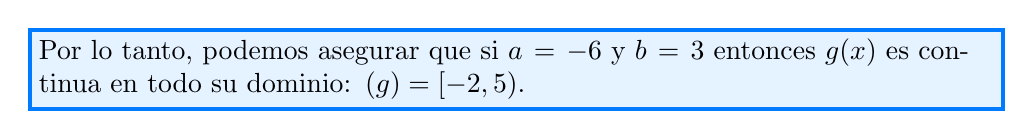
\begin{tikzpicture}
	\node[draw=lightblue, fill=lightblue!10, line width=1.5, text width=\linewidth] {Por lo tanto, podemos asegurar que si $a=-6$ y $b=3$ entonces $g(x)$ es continua en todo su dominio: $\dom(g)=[-2,5)$.};
\end{tikzpicture}
\end{enumerate}
\item \lb{Calcular el siguiente límite: \[ \lim_{x\to0}\dfrac{\sqrt{1+x}-\sqrt{1-x}}{x} \]}
$\lim_{x\to0}\dfrac{\sqrt{1+x}-\sqrt{1-x}}{x}=\left(\dfrac{0}{0}\right)=\left\{\begin{array}{l}
	\text{multiplicaremos y dividiremos}\\
	\text{por el conjugado de las raíces}
\end{array}\right\}=\lim_{x\to0}\dfrac{(\sqrt{1+x}-\sqrt{1-x})\cdot(\sqrt{1+x}-\sqrt{1-x})}{x(\sqrt{1+x}+\sqrt{1-x})}\linebreak=\lim_{x\to0}\dfrac{(\sqrt{1+x})^2-(\sqrt{1-x})^2}{x(\sqrt{1+x}+\sqrt{1-x})}=\lim_{x\to0}\dfrac{(\cancel{1}-x)-(\cancel{1}-x)}{x(\sqrt{1+x}+\sqrt{1-x})}=\lim_{x\to0}\dfrac{2\cancel{x}}{\cancel{x}(\sqrt{1+x}+\sqrt{1-x})}=\dfrac{2}{2}=\bboxed{1}$
\item \lb{Calcular el siguiente límite: \[ \lim_{x\to+\infty}\dfrac{3x^2+2}{x^2+3x+5} \]}

\begin{minipage}{0.5\textwidth}
	$\lim_{x\to+\infty}\dfrac{3x^2+2}{x^2+4x+5}=\left(\dfrac{\infty}{\infty}\right)=\lim_{x\to+\infty}\dfrac{\frac{3x^2}{x^2}+\frac{2}{x^2}}{\frac{x^2}{x^2}+\frac{3x}{x^2}+\frac{5}{x^2}}=\lim_{x\to+\infty}\dfrac{3+\tozero{\frac{2}{x^2}}}{1+\tozero{\frac{3}{x}}+\tozero{\frac{5}{x^2}}}=\bboxed{3}$
\end{minipage}\qquad\begin{minipage}{0.4\textwidth}
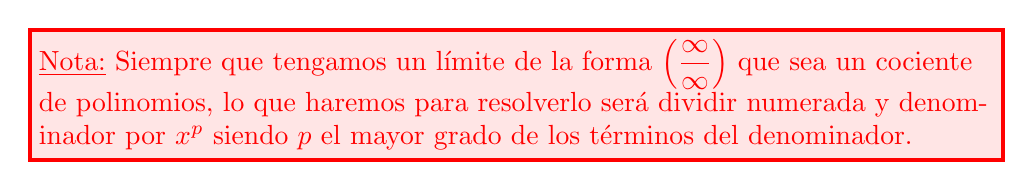
\begin{tikzpicture}
	\node[red, draw=red, fill=red!10, line width=1.5, text width=\linewidth] {\underline{Nota:} Siempre que tengamos un límite de la forma $\left(\dfrac{\infty}{\infty}\right)$ que sea un cociente de polinomios, lo que haremos para resolverlo será dividir numerada y denominador por $x^p$ siendo $p$ el mayor grado de los términos del denominador.};
\end{tikzpicture}
\end{minipage}
\item \lb{Calcular el siguiente límite: \[ \lim_{x\to+\infty}\dfrac{3x}{x^2+2} \]}
$\lim_{x\to+\infty}\dfrac{3x}{x^2+2}=\left(\dfrac{\infty}{\infty}\right)=\lim_{x\to+\infty}\dfrac{\frac{3x}{x^2}}{\frac{x^2}{x^2}+\frac{2}{x^2}}=\lim_{x\to+\infty}\dfrac{\tozero{\frac{3}{x}}}{1+\tozero{\frac{2}{x^2}}}=\dfrac{0}{1}=\bboxed{0}$
\item \lb{Calcular el siguiente límite: \[ \lim_{x\to+\infty}\left(\dfrac{x+1}{x-1}\right)^x \]}
\begin{minipage}{0.55\textwidth}
	$\lim_{x\to+\infty}\left(\dfrac{x+1}{x-1}\right)^x=(1^\infty)=e^{\displaystyle\lim_{x\to0}x\left[\frac{x+1}{x-1}-1\right]}=\lb{(\ast)}=\bboxed{e^2}$
	
	\lb{\underline{Base:}\\
	$\lim_{x\to+\infty}\dfrac{x+1}{x-1}=\lim_{x\to+\infty}\dfrac{\frac{x}{x}+\tozero{\frac{1}{x}}}{\frac{x}{x}-\tozero{\frac{1}{x}}}=1$}
	
\end{minipage}\qquad\begin{minipage}{0.4\textwidth}
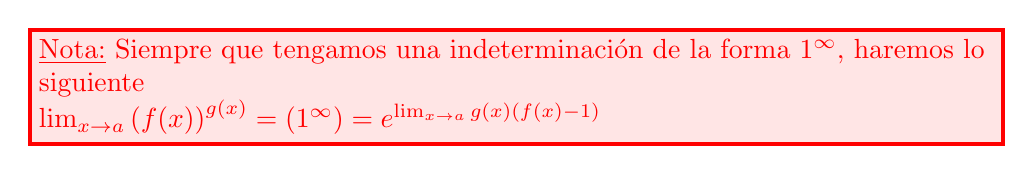
\begin{tikzpicture}
	\node[red, draw=red, fill=red!10, line width=1.5, text width=\linewidth] {\underline{Nota:} Siempre que tengamos una indeterminación de la forma $1^\infty$, haremos lo siguiente\\
	$\lim_{x\to a}\left(f(x)\right)^{g(x)}=(1^\infty)=e^{\lim_{x\to a}g(x)\left(f(x)-1\right)}$};
\end{tikzpicture}
\end{minipage}
	
	$\lb{(\ast)=} \lim_{x\to+\infty}x\left[\dfrac{\cancel{x}+1-\cancel{x}+1}{x-1}\right]=\lim_{x\to+\infty}\dfrac{2x}{x-1}=\left(\dfrac{\infty}{\infty}\right)\dfrac{\frac{2x}{x}}{\frac{x}{x}-\tozero{\frac{1}{x}}}=2$
	
\item \lb{Calcular el siguiente límite: \[ \lim_{x\to+\infty}(\sqrt{x^2+1}-\sqrt{x^2-4}) \]}

$\lim_{x\to+\infty}(\sqrt{x^2+1}-\sqrt{x^2-4})=(\infty-\infty)=\lim_{x\to+\infty} \dfrac{(\sqrt{ x^{2}+1 })-(\sqrt{ x^{2}-4 })\cdot(\sqrt{ x^{2}+1 })+(\sqrt{ x^{2}-4 })}{(\sqrt{ x^{2}+1 })+(\sqrt{ x^{2}-4 })}=\linebreak\lim_{ x \to +\infty }\dfrac{(\sqrt{ x^{2}+1 })^{2}-(\sqrt{ x^{2}-4 })^2}{\sqrt{ x^{2}+1 }+\sqrt{ x^{2}-4 }}=\lim_{ x \to +\infty }\dfrac{(\cancel{x^{2}}+1)-(\cancel{x^{2}}-4)}{\sqrt{ x^{2}+1 }+\sqrt{ x^{2}-4  }}=\lim_{ x \to +\infty }\frac{5}{\sqrt{ x^{2}+1 }+\sqrt{ x^{2}-4 }}=\lim_{ x \to +\infty }\dfrac{5}{+\infty}=\bboxed{0}$
\item \lb{Estudiar la continuidad de la siguiente función: \[ f(x)=\begin{cases}
		\dfrac{1}{e^{\frac{1}{x-1}}+1} & \text{si }x\neq1\\
		1 & \text{si }x=1
	\end{cases} \]}

$\forall x\neq1\longrightarrow f(x)$ es continua por ser un cociente de funciones continuas con denominador distinto de cero.

Veamos si $f(x)$ es continua en $x=1$:

\begin{center}
	$\begin{rcases}
		\lim_{x\to1^-}\dfrac{1}{e^{\frac{1}{x-1}}+1}=\frac{1}{e^{\frac{1}{0^-}}+1}=\dfrac{1}{e^{-\infty}+1}=\left\{e^{-\infty}=\dfrac{1}{e^{+\infty}}=\dfrac{1}{+\infty}=0\right\}=\dfrac{1}{1}=1\\
		\lim_{x\to1^+}=\dfrac{1}{e^{\frac{1}{x-1}}+1}=\dfrac{1}{e^{\frac{1}{0^+}}+1}=\dfrac{1}{e^{+\infty}+1}=\dfrac{1}{+\infty}=0
	\end{rcases}~~$\begin{minipage}{0.3\textwidth}
	Como los límites laterales no son iguales, entonces no existe el límite en $x=1\longrightarrow f(x)$ no es continua en $x=1$.
	\end{minipage}
\end{center}
En concreto podemos asegurar que $f(x)$ presenta en $x=1$ una discontinuidad inevitable de salto finito o de 1ª especie.

\fcolorbox{lightblue}{lightblue!10}{Por lo tanto, la conclusión es que $f(x)$ es continua $\forall x\in\R-\{1\}$.}
\item \lb{Calcular \[ \lim_{x\to+\infty}\left(\dfrac{x^2-3x+6}{x^2+4x-1}\right)^{\dfrac{x^3}{1-x^2}} \]}

$\lim_{x\to+\infty}\left(\dfrac{x^2-3x+6}{x^2+4x-1}\right)^{\dfrac{x^3}{1-x^2}}=\lb{(\ast)}=\left(1^\infty\right)=\lb{(\ast\ast)}$

$\lb{(\ast)}\begin{cases}
	\text{\underline{Base:} }\lim_{x\to+\infty}\left(\dfrac{x^2-3x+6}{x^2+4x-1}\right)=\left(\dfrac{\infty}{\infty}\right)=\lim_{x\to+\infty}\dfrac{\frac{x^2}{x^2}-\frac{3x}{x^2}+\frac{6}{x^2}}{\frac{x^2}{x^2}+\frac{4x}{x^2}-\frac{1}{x^2}}=\lim_{x\to+\infty}\dfrac{1-\tozero{\frac{3}{x}}+\tozero{\frac{6}{x^2}}}{1+\tozero{\frac{4}{x}}-\tozero{\frac{1}{x^2}}}=1\\
	\text{\underline{Exponente:} }\lim_{x\to+\infty}\dfrac{x^3}{1-x^2}=\left(\dfrac{\infty}{\infty}\right)=\lim_{x\to+\infty}\dfrac{\frac{x^3}{x^3}}{\frac{1}{x^2}-\frac{x^2}{x^2}}=\lim_{x\to+\infty}\dfrac{x}{\tozero{\frac{1}{x^2}}-1}=\dfrac{\infty}{-1}=-\infty
\end{cases}$

$\lb{(\ast\ast)=}e^{\displaystyle\lim_{x\to+\infty}\dfrac{x^3}{1-x^2}\left[\dfrac{x^2-3x+6}{x^2+2x-1}-1\right]}=\bboxed{e^7}$

$\lim_{x\to+\infty}\dfrac{x^3}{1-x^2}\left[\dfrac{x^2-3x+6}{x^2+2x-1}-1\right]=\lim_{x\to+\infty}\dfrac{x^3}{1-x^2}\left[\dfrac{\cancel{x^2}-3x+6-\cancel{x^2}-4x+1}{x^2+4x-1}\right]=\lim_{x\to+\infty}\dfrac{x^3}{1-x^2}\cdot\dfrac{-7x+7}{x^2+4x-1}=\linebreak\lim_{x\to+\infty}\dfrac{-7x^3+7x^3}{x^2+4x-1-x^4-4x^3+x^2}=\lim_{x\to+\infty}\dfrac{-7x^4+7x^3}{-x^4-4x^3+2x^2+4x-1}=\left(\dfrac{\infty}{\infty}\right)=\lim_{x\to+\infty}\dfrac{-\frac{7}{x^4}+\frac{7x^3}{x^4}}{-\frac{x^4}{x^4}-\frac{4x^3}{x^4}+\frac{2x^2}{x^4}+\frac{4x}{x^4}-\frac{1}{x^4}}=\lim_{x\to+\infty}\frac{-7+\tozero{\frac{7}{x}}}{-1-\tozero{\frac{4}{x}}+\tozero{\frac{2}{x^2}}+\tozero{\frac{4}{x^3}}-\tozero{\frac{1}{x^4}}}=\frac{-7}{-1}=7$ 
\item \lb{Calcular el siguiente límite: \[ \lim_{x\to0}x\sin\dfrac{1}{x} \]}

\begin{minipage}{0.45\textwidth}
	Como tenemos:
	\begin{itemize}
		\item $\lim_{x\to 0}x=0$
		\item $\sin\dfrac{1}{x}$ es una función acotada ya que siempre ocurrirá que $-1\le\sin\dfrac{1}{x}\le1$
	\end{itemize}
	Por lo tanto por el teorema del encaje (Sándwich), tendremos que: \[ \bboxed{\lim_{x\to0}x\sin\left(\dfrac{1}{x}\right)=0} \]
\end{minipage}\qquad\begin{minipage}{0.45\textwidth}
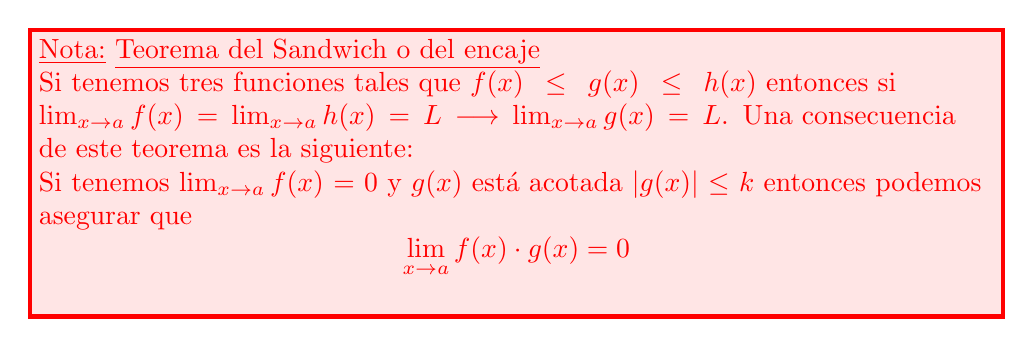
\begin{tikzpicture}
	\node[red, draw=red, fill=red!10, line width=1.5, text width=\linewidth] {\underline{Nota:} \underline{Teorema del Sandwich o del encaje}\\ Si tenemos tres funciones tales que $f(x)\le g(x)\le h(x)$ entonces si $\lim_{x\to a}f(x)=\lim_{x\to a}h(x)=L\longrightarrow\lim_{x\to a}g(x)=L$. Una consecuencia de este teorema es la siguiente:
	
	Si tenemos $\lim_{x\to a}f(x)=0$ y $g(x)$ está acotada $\left|g(x)\right|\le k$ entonces podemos asegurar que \[ \lim_{x\to a}f(x)\cdot g(x)=0 \]};
\end{tikzpicture}
\end{minipage}
\item \lb{Calcular el límite \[ \lim_{x\to+\infty}\dfrac{\sin(x)}{x} \]}
$\lim_{x\to+\infty}\dfrac{\sin(x)}{x}=\lim_{x\to+\infty}\dfrac{1}{x}\cdot\sin(x)$

Como se cumple que: 
\begin{itemize}
	\item $\lim_{x\to+\infty}=0$
	\item La función $\sin(x)$ está acotada, ya que $-1\le\sin(x)\le1$
\end{itemize}
Aplican el teorema del encaje (Sándwich), tendremos que: \[ \bboxed{\lim_{x\to+\infty}\dfrac{1}{x}\cdot\sin(x)=0} \]
\item \lb{Calcular el siguiente límite: \[ \lim_{x\to0}\dfrac{\sin(x)}{x} \]}
\begin{minipage}{0.32\textwidth}
	Aplicando la equivalencia: $\sin(x)\leadsto_0 x$ podemos decir que: \[ \lim_{x\to0}\dfrac{\sin(x)}{x}=\lim_{x\to0}\dfrac{x}{x}=\bboxed{1} \]
\end{minipage}\qquad\begin{minipage}{0.63\textwidth}
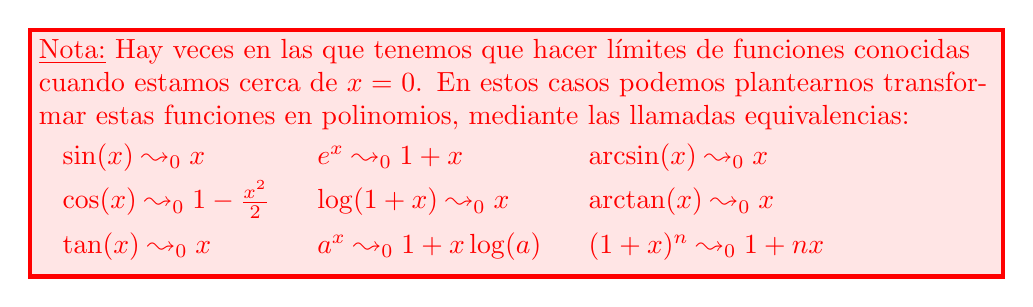
\begin{tikzpicture}
	\node[red, draw=red, fill=red!10, line width=1.5, text width=\linewidth] {\underline{Nota:} Hay veces en las que tenemos que hacer límites de funciones conocidas cuando estamos cerca de $x=0$. En estos casos podemos plantearnos transformar estas funciones en polinomios, mediante las llamadas equivalencias:\\
	$\begin{array}{lll}
		\sin(x)\leadsto_0x &e^x\leadsto_01+x  & \arcsin(x)\leadsto_0 x\\
		\cos(x)\leadsto_01-\frac{x^2}{2} & \log(1+x)\leadsto_0 x & \arctan(x)\leadsto_0 x\\
		\tan(x)\leadsto_0 x & a^x\leadsto_0 1+x\log(a) & (1+x)^n\leadsto_01+nx\\
	\end{array}$};
\end{tikzpicture}
\end{minipage}
\item \lb{Calcular el siguiente límite: \[ \lim_{x\to0}\dfrac{1-\cos(2x)}{3x\sin(2x)} \]}

$\lim_{x\to0}\dfrac{1-\cos(2x)}{3x\sin(2x)}=\left(\dfrac{0}{0}\right)=\lb{(\ast)}$

Resolveremos este límite aplicando equivalencias:\[ \begin{array}{rl}
	\sin(x)\leadsto_0 x\xrightarrow{\qquad} & \sin(2x)\leadsto_0(2x)\\
	\cos(x)\leadsto_01-\frac{x^2}{2}\xrightarrow{\qquad} & \cos(2x)\leadsto_0 1-\frac{(2x)^2}{2}=1-2x^2
\end{array} \] $\lb{(\ast)=}\lim_{x\to0}\dfrac{\cancel{1}-(\cancel{1}-2x^2)}{3x\cdot(2x)}=\lim_{x\to0}\dfrac{2\cancel{x^2}}{6\cancel{x^2}}=\bboxed{\dfrac{1}{3}}$
\item \lb{Calcular el límite $\lim_{x\to0}\dfrac{\sin^2(x)\tan^3(3x)}{(1-\cos^2(x))\cdot(e^x-1)^3}$}

$\lim_{x\to0}\dfrac{\sin^2(x)\tan^3(3x)}{\lbb{(1-\cos^2(x))}{\sin^2(x)}\cdot(e^x-1)^3}=\lim_{x\to0}\dfrac{\cancel{\sin^2(x)}\cdot\tan^3(3x)}{\cancel{\sin^2(x)}\cdot(e^x-1)^3}=\lim_{x\to0}\dfrac{\tan^3(3x)}{(e^x-1)^3}=\left(\dfrac{0}{0}\right)=\lb{(\ast)}$

Aplicaremos equivalencias para resolver este límite: \[ \begin{array}{l}
	\tan(x)\leadsto_0 x\longrightarrow\bboxed{\tan(3x)\leadsto_03x}\\
	\bboxed{e^x\leadsto_01+x}
\end{array} \]$\lb{(\ast)=}\lim_{x\to0}\dfrac{(3x)^3}{(1+x-1)^3}=\lim_{x\to0}\dfrac{27x^3}{x^3}=\bboxed{27}$

\item \lb{Para calcular \[ \lim_{x\to0^+}e^{\frac{2}{3-\ln x}} \]}
\begin{minipage}{0.4\textwidth}
	$\lim_{x\to0^+}=(0^0)=\lim_{x\to0^+}e^{\log x^{\frac{2}{3-\ln x}}}=\lim_{x\to0^+}e^{\frac{2}{3-\ln x}\cdot\ln x}=e^{\lim_{x\to0^+}\frac{2\ln x}{3-\ln x}}=\lb{(\ast)}=\bboxed{e^{-2}}$
	
	\lb{\underline{Exponente:} $\lim_{x\to0^+}\dfrac{2}{3-\ln x}=\left\{\ln(0^+) =-\infty\right\}=\dfrac{2}{\infty}=0$}
	
	$\lb{(\ast)=}\lim_{x\to0^+}\dfrac{2\ln x}{3-\ln x}=\left(\dfrac{\infty}{\infty}\right)=\lim_{x\to0^+}\dfrac{2\frac{\cancel{\ln x}}{\cancel{\ln x}}}{\frac{3}{\ln x}-\frac{\cancel{\ln x}}{\cancel{\ln x}}}=\lim_{x\to0^+}\dfrac{2}{\tozero{\frac{3}{\ln x}}-1}=-2$
\end{minipage}\qquad\begin{minipage}{0.45\textwidth}
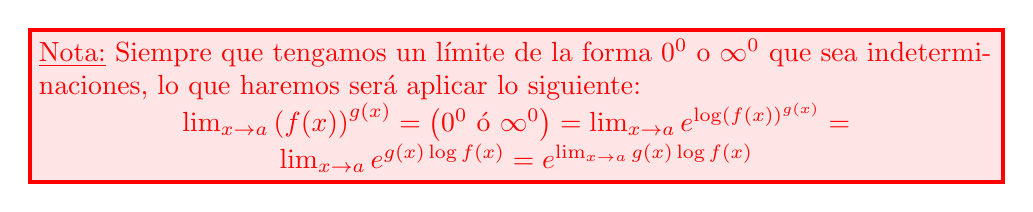
\begin{tikzpicture}
	\node[red, draw=red, fill=red!10, line width=1.5, text width=\linewidth] {\underline{Nota:} Siempre que tengamos un límite de la forma $0^0$ o $\infty^0$ que sea indeterminaciones, lo que haremos será aplicar lo siguiente: \begin{center}
			$\lim_{x\to a}\left(f(x)\right)^{g(x)}=\left(0^0\text{ ó }\infty^0\right)=\lim_{x\to a}e^{\log\left(f(x)\right)^{g(x)}}=\linebreak\lim_{x\to a}e^{g(x)\log f(x)}=e^{\lim_{x\to a}g(x)\log f(x)}$
	\end{center}};
\end{tikzpicture}
\end{minipage}

\item \lb{Para calcular \[ \lim_{x\to+\infty}(5x^3)^{\dfrac{1}{\ln(x^2)}} \]}
$\lim_{x\to+\infty}(5x^3)^{\frac{1}{\ln x^2}}=(\infty^0)=\lim_{x\to+\infty}e^{\ln(5x^3)^{\frac{1}{\ln x^2}}}=\lim_{x\to+\infty}e^{\frac{1}{\ln x^2}\ln(5x^3)}=e^{\lim_{x\to+\infty}\frac{\ln(5x^3)}{\ln x^2}}=\lb{(\ast)}=e^{\frac{3}{2}}$

$\lb{(\ast)}=\lim_{x\to+\infty}\dfrac{\ln(5x^3)}{\ln x^2}=\lim_{x\to+\infty}\dfrac{\ln 5+\ln x^3}{\ln x^2}=\lim_{x\to+\infty}\dfrac{\ln 5+3\ln x}{2\ln x}=\left(\dfrac{\infty}{\infty}\right)=\lim_{x\to+\infty}\dfrac{\tozero{\frac{\ln 5}{\ln x}}+3\frac{\cancel{\ln x}}{\cancel{\ln x}}}{2\frac{\cancel{\ln x}}{\cancel{\ln x}}}=\dfrac{3}{2}$
\item \lb{Calcular el siguiente límite: \[ \lim_{x\to+\infty}\dfrac{\ln(2x^3+5x^2+6x+2)}{\ln(x^2+5)} \]}

\begin{minipage}{0.6\textwidth}
{\small	$\lim_{ x \to +\infty }\dfrac{\ln(2x^{3}+5x^{2}+6x+2)}{\ln(x^{2}+5)}=\left( \frac{\infty}{\infty} \right)=\lim_{ x \to +\infty }\dfrac{\ln\left( x^{3}\left( 2+\frac{5}{x}+\frac{6}{x^{2}}+\frac{2}{x^{3}} \right) \right)}{\ln\left( x^{2}\left( 1+\frac{5}{x^{2}} \right) \right)}=\lim_{ x \to +\infty }\dfrac{\ln(x^{3})+\ln\left( 2+\frac{5}{x}+\frac{6}{x^{2}}+\frac{2}{x^{3}} \right)}{\ln(x^{2})+\ln\left( 1+\frac{5}{x^{2}} \right)}=\lim_{ x \to +\infty }\dfrac{3\ln x+\ln\left( 2+\frac{5}{x}+\frac{6}{x^{2}}+\frac{2}{x^{3}} \right)}{2\ln x+\ln\left( 1+\frac{5}{x^{2}} \right)}=\left( \frac{\infty}{\infty} \right)=\lim_{ x \to +\infty }\dfrac{\frac{3\cancel{\ln x}}{\cancel{\ln x}}+\cancelto{0}{\frac{\ln\left( 2+\frac{5}{x}+\frac{6}{x^{2}}+\frac{2}{x^{3}} \right)}{\ln x}}}{\frac{2\ln x}{\ln x}+\cancelto{0}{\frac{\ln\left( 1+\frac{5}{x^{2}} \right)}{\ln x}}}=\bboxed{\frac{3}{2}}$}
\end{minipage}\qquad\begin{minipage}{0.3\textwidth}
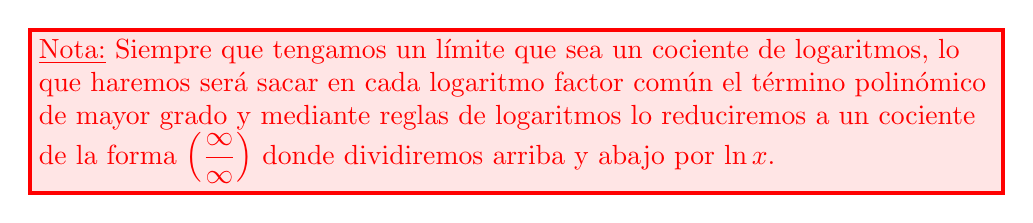
\begin{tikzpicture}
	\node[red, draw=red, fill=red!10, line width=1.5, text width=\linewidth] {\underline{Nota:} Siempre que tengamos un límite que sea un cociente de logaritmos, lo que haremos será sacar en cada logaritmo factor común el término polinómico de mayor grado y mediante reglas de logaritmos lo reduciremos a un cociente de la forma $\left(\dfrac{\infty}{\infty}\right)$ donde dividiremos arriba y abajo por $\ln x$.};
\end{tikzpicture}
\end{minipage}
\item \lb{Si queremos calcular $A$ para que la función \[ f(x)=\begin{cases}
		\dfrac{x^2-4}{x-2} & \text{si }x\neq2\\
		A & \text{si }x=2
	\end{cases} \] sea continua en el punto $x_0=2$ lo que tenemos que hacer es calcular.}

\begin{minipage}{0.5\textwidth}
	\begin{itemize}[leftmargin=*]
		\item Veamos si existe el límite en $x_0=2$. \[ \lim_{x\to 2}\dfrac{x^2-5}{x-2}=\left(\dfrac{0}{0}\right)=\lim_{x\to2}\dfrac{\cancel{(x-2)}(x+2)}{\cancel{x-2}}=4\longrightarrow\lim_{x\to2}f(x)=4 \]
		\item Como podemos ver en $f(x)$, existe $f(2)$ y vale $f(2)=A$.
		\item Para que $f(x)$ sea continua en $x=2$, debe verificarse que $\lim_{x\to2}f(x)=f(2)$ \[ \bboxed{A=4} \]
	\end{itemize}
\end{minipage}\qquad\begin{minipage}{0.4\textwidth}
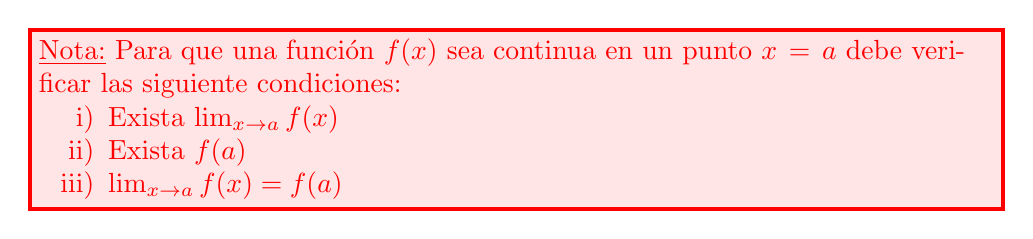
\begin{tikzpicture}
	\node[red, draw=red, fill=red!10, line width=1.5, text width=\linewidth] {\underline{Nota:} Para que una función $f(x)$ sea continua en un punto $x=a$ debe verificar las siguiente condiciones:
	\begin{enumerate}[label=\color{red}\roman*)]
		\item Exista $\lim_{x\to a}f(x)$
		\item Exista $f(a)$\\
		\item $\lim_{x\to a}f(x)=f(a)$
		\end{enumerate}};
\end{tikzpicture}
\end{minipage}
\item \lb{Sea $k\in\Z$. Si queremos estudiar la continuidad de la función en el punto $x_0=\pi$ \[ f(x)=\begin{cases}
		\dfrac{x}{\sin x} & \text{si }x\neq k\pi\\
		1 & \text{si }x=k\pi,
	\end{cases} \]}

Para estudiar la continuidad de $f(x)$ en $x=\pi$ debemos hacer lo siguiente:

$\lim_{x\to\pi}\dfrac{x}{\sin x}=\left(\dfrac{\pi}{0}\right)=\begin{cases}
	\lim_{x\to\pi^-}\dfrac{x}{\sin x}=\dfrac{\pi}{0^+}=+\infty
	\lim_{x\to\pi^+}\dfrac{x}{\sin x}=\dfrac{\pi}{0^-}=-\infty
\end{cases}$

\begin{tikzpicture}[ >=latex, scale=0.8, baseline=(current bounding box.center)]
	\begin{axis}[xmin=-1, xtick=\empty, ytick=\empty, axis lines=center, xmax=2.2*pi, xscale=1.5]
		\addplot[samples=150, lightblue, domain=0:2*pi, line width=1.5] {sin(deg(x))};
		\draw[lightblue] (axis cs:pi, 0.1) -- (axis cs: pi, -0.1) node[below] {$\pi$};
	\end{axis}
\end{tikzpicture}\qquad\begin{minipage}{0.4\textwidth}
No es continua en $x_0=\pi$ en concreto, podemos asegurar que $f(x)$ presenta una discontinuidad inevitable de salto infinito en $x_0=\pi$. Hay, por lo tanto, una asíntota vertical $x_0=\pi$.
\end{minipage}
\item \lb{Estudiar la continuidad de la función \[ f(x)=\begin{cases}
		3 & \text{si }x<2\\
		x^2 & \text{x }\ge2
	\end{cases} \]en el punto $x_0=2$.}

Para estudiar la continuidad de $f(x)$ en el punto $x_0=2$, debemos: 
\begin{enumerate}[label=\roman*)]
	\item Estudiaremos la existencia del límite de $f(x)$ en $x_0=2$. 
	\begin{center}
		$\lim_{x\to2}f(x)=\begin{cases}
			\lim_{x\to2^-}3=3\\
			\lim_{x\to 2^+}x^2=4
		\end{cases}\longrightarrow\nexists\lim_{x\to 2} f(x)~~$\begin{minipage}[t]{0.4\textwidth}
		Por lo tanto $f(x)$ no es continua en $x=2$ en concreto presenta una discontinuidad inevitable de salto finito o de 1ª especie.
		\end{minipage}
	\end{center}
\end{enumerate}
\item \lb{Estudiar la continuidad de la función \[ f(x)=\begin{cases}
		\dfrac{\sin\frac{1}{x-1}}{e^{\frac{1}{x-1}}+1} & \text{si }x\neq1\\
		0 & \text{si }x=1
	\end{cases} \]en el punto $x_0=1$.}

Para estudiar la continuidad, debemos hacer lo primero el límite en $x_0=1$.
\[ \lim_{x\to1}f(x)=\begin{cases}
	\lim_{x\to1^-}\dfrac{\sin\left(\frac{1}{x-1}\right)}{e^{\frac{1}{x-1}}+1}=\dfrac{\sin\left(\frac{1}{0^-}\right)}{e^{\frac{1}{0^-}+1}}=\dfrac{\overbrace{\sin(-\infty)}^{\mathrm{oscilante}}}{\tozero{e^{-\infty}}+1}=\nexists\lim\text{ ya que es oscilante}\\
	\lim_{x\to1^+}\dfrac{\sin\left(\frac{1}{x-1}\right)}{e^{\frac{1}{x-1}}+1}=\dfrac{\sin\left(\frac{1}{0^+}\right)}{e^{\frac{1}{0^+}}+1}=\dfrac{\sin(+\infty)}{e^{+\infty}+1}=\dfrac{\sin(+\infty)}{+\infty}=0\text{ (Teorema del Sandwich)}
\end{cases} \]
No existe el límite ya que hay un límite lateral que no existe $\longrightarrow f(x)$ no es continua en $x_0=1$.
\item \lb{Consideremos las funciones \[ f(x)=e^{-x}x\hspace{2cm}g(x)=\dfrac{1}{x} \]Estudiar la continuidad de la función $f\circ g$}

La composición de funciones $f\circ g$, consiste en realizar la función $g(x)$, y donde esta termine comenzaremos $f(x)$:

\begin{center}
	\begin{tikzcd}[nodes={anchor=west}, row sep=tiny]
		\mathbb{R} \arrow[rr, "g"] &  & \mathbb{R} \arrow[rr, "f"] &  & \mathbb{R}                                                                               \\
		x \arrow[rr]               &  & g(x)                       &  &                                                                                          \\
		&  & \frac{1}{x} \arrow[rr]    &  & f\left(\dfrac{1}{x}\right)=e^{-\frac{1}{x}}\cdot\frac{1}{x}=\dfrac{e^{-\frac{1}{x}}}{x} \\
		&  &                            &  & f(x)=e^{-x}\cdot x                                                                      
	\end{tikzcd}
\end{center}

Por lo tanto, tenemos que: $\bboxed{(f\circ g)=\dfrac{e^{-\frac{1}{x}}}{x}}$. 

Por lo tanto podemos asegurar que $(f\circ g)$ es continua en todos los $\R$ salvo en $x=0$, donde $\nexists(f\circ g)(0)$

\item \lb{Dadas las funciones reales $f(x)=\sin x$ y $g(x)=\sqrt{x}$. Calcular las expresiones de $g\circ f$ y $f\circ g$.}

Comenzamos calculando $g\circ f$: 
\begin{center}
	\begin{tikzcd}[nodes={anchor = west}, row sep = tiny]
		\mathbb{R} \arrow[r, "f"] & \mathbb{R} \arrow[r, "g"] & \mathbb{R}         \\
		x \arrow[r]               & f(x) \arrow[r]            & g\left(f(x)\right) \\
		x \arrow[r]               & \sin x \arrow[r]          & \sqrt{\sin x}     
	\end{tikzcd}$\longrightarrow\bboxed{(g\circ f)(x)=\sqrt{\sin x}}$
\end{center}
Calcularemos ahora $f\circ g$:
\begin{center}
		\begin{tikzcd}[nodes={anchor = west}, row sep = tiny]
		\mathbb{R} \arrow[r, "g"] & \mathbb{R} \arrow[r, "f"] & \mathbb{R}         \\
		x \arrow[r]               & g(x) \arrow[r]            & f\left(g(x)\right) \\
		x \arrow[r]               & \sqrt{x} \arrow[r]          & \sin\left(\sqrt{x}\right)
	\end{tikzcd}$\longrightarrow\bboxed{(f\circ g)(x)=\sin(\sqrt{x})}$
\end{center}
\item \lb{Para calcular el límite \[ \lim_{x\to2}\dfrac{(x^2-x-2)^{20}}{(x^3-12x+16)^{10}}. \]}

$\begin{array}{l}
	\lim_{x\to2}\dfrac{(x^2-x-2)^{20}}{(x^3-12x+16)^{10}}=\left(\dfrac{0}{0}\right)=\lb{(\ast)}\\
	x^2-x-2=0\longrightarrow x=\dfrac{1\pm\sqrt{1+8}}{2}=\dfrac{1\pm3}{2}\begin{cases}
		2\\
		-1
	\end{cases}\longrightarrow(x^2-x-2)=(x-2)(x+1)\\
	x^3-12x+16=0
\end{array}$

$\begin{array}{c|cccc}
	& 1 & 0 & -12 & 16 \\
	2 &  & 2 & 4 & -16 \\ \hline
	& 1 & 2 & -8 & \multicolumn{1}{|c|}{0} \\ \cline{5-5}
	2 &  & 2 & 8 &  \\ \hline
	& 1 & 4 & \multicolumn{1}{|c|}{0} &  \\ \cline{4-4}
\end{array}\qquad(x^3-12x+16)=(x-2)^2(x+4)$

$\lb{(\ast)=}\lim_{x\to2}\dfrac{[(x-2)(x+1)^{20}]}{[(x-2)^2(x+4)]^{10}}=\lim_{x\to2}\dfrac{\cancel{(x-2)^{20}}\cdot(x+1)^{20}}{\cancel{(x-2)^{20}}\cdot(x+4)^{10}}=\dfrac{3^{20}}{6^{10}}=\dfrac{3^{20}}{2^{10}\cdot3^{10}}=\bboxed{\dfrac{3^{10}}{2^{10}}}$
\item \lb{Calcular el siguiente límite: \[ \lim_{x\to x_0}\dfrac{\sqrt{x}-\sqrt{x_0}}{x-x_0}. \]}

$\lim_{x\to x_0}\dfrac{\sqrt{x}-\sqrt{x_0}}{x-x_0}=\left(\dfrac{0}{0}\right)=\lim_{x\to x_0}\dfrac{(\sqrt{x}-\sqrt{x_0})\cdot(\sqrt{x}+\sqrt{x_0})}{(x-x_0)(\sqrt{x}+\sqrt{x_0})}=\lim_{x\to x_0}\dfrac{\cancel{x-x_0}}{\cancel{(x-x_0)}(\sqrt{x}-\sqrt{x_0})}=\lim_{x\to x_0}\dfrac{1}{\sqrt{x}+\sqrt{x_0}}=\bboxed{\dfrac{1}{2\sqrt{x_0}}}$

\item \lb{Calcula la correspondencia inversa de las funciones:}

$\db{y=\sqrt{\dfrac{x-1}{x+2}}}$

La función inversa es aquella que verifica que si $f(x)\longrightarrow x=f^{-1}(y)$

$\begin{array}{l}
	y=\sqrt{\dfrac{x-1}{x+2}}\longrightarrow\dfrac{x-1}{x+2}=y^2\longrightarrow(x-1)=y^2(x+2)\\
	x-1=xy^2+2y^2\longrightarrow x-xy^2=1+2y^2\longrightarrow x(1-y^2)=1+2y^2\\
\end{array}$\[ x=\dfrac{1+2y^2}{1-y^2}\longrightarrow\bboxed{x\cdot f^{-1}(y)=\dfrac{1+2y^2}{1-y^2}} \]
\item \lb{Calcula la correspondencia inversa de las funciones:}

$\db{y=\dfrac{2+\sqrt{x}}{2-\sqrt{x}}}$

La función invertible que verifica que si $y=f(x)\longrightarrow x=f^{-1}(y)$

$\begin{array}{l}
	y=\dfrac{2+\sqrt{x}}{2-\sqrt{x}}\longrightarrow(2-\sqrt{x})y=2+\sqrt{x}\longrightarrow2t-t\sqrt{x}=2+\sqrt{x}\longrightarrow2y-2=2\sqrt{x}+\sqrt{x}\\
	2y-2=(y+1)\sqrt{x}\longrightarrow\sqrt{x}=\dfrac{2y-2}{y+1}\longrightarrow x=\left(\dfrac{2y-2}{y+1}\right)^2\longrightarrow\bboxed{x=f^{-1}(y)=\left(\dfrac{2y-2}{y+1}\right)^2}
\end{array}$
\item \lb{Calcula el dominio de las siguiente funciones:}

$\db{f(x)=\dfrac{x}{x+1}}$

Como $f(x)$ está definida mediante un cociente, entonces tenemos que su denominador no puede ser cero \[ \begin{array}{l}
	x+1=0\longrightarrow x=-1\\
	\bboxed{\dom(f)=\R-\{-1\}}
\end{array} \]
\item \lb{Calcula el dominio de las siguientes funciones:}

$\db{g(x)=\dfrac{x+3}{x^2-4}}$

Como tenemos un cociente, el denominador no puede ser cero. \[ \begin{array}{l}
	x^2-4=0\longrightarrow x^2=4\longrightarrow x=\pm2\\
	\bboxed{\dom(g(x))=\R-\{-2,\,2\}}
\end{array} \]
\item \lb{Calcula el dominio de las siguientes funciones:}

$\db{l(x)=\sqrt{\dfrac{x-1}{x+2}}}$
\begin{itemize}
	\item Lo primero que tenemos es un cociente, el cual no puede tener el denominador igual a cero \begin{center}
		$x+2=0\longrightarrow\bboxed{x=-2}$ No está en el dominio
	\end{center}
	\item Como tenemos una raíz cuadrada, entonces lo de dentro no puede ser negativo:
	
	$\dfrac{x-1}{x+2}\ge0$
	
		\begin{center}
		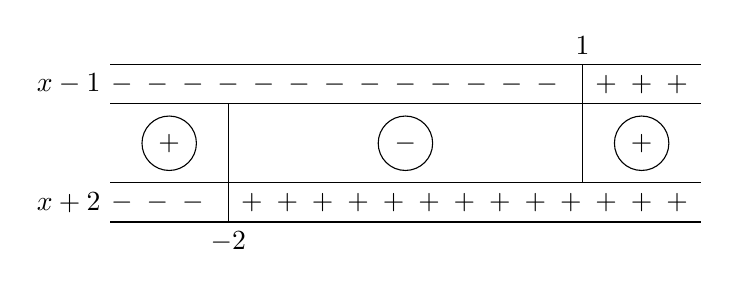
\begin{tikzpicture}[xscale=1.5]
			\draw (-3,0) -- (2,0)
			(-3,-0.5) -- (2,-0.5)
			(-3,-1.5) -- (2,-1.5)
			(-3,-2) -- (2,-2);
			\node[left] at (-3,-0.25-1.5) {$x+2$};
			\node[left] at (-3,-1.75+1.5) {$x-1$};
			\foreach \x in {-2.9, -2.6, ..., -2.1}{
				\node at (\x, -0.25-1.5) {$-$};
			}
			\foreach \x in {-2.9, -2.6, ..., 0.8}{
				\node at (\x, -1.75+1.5) {$-$};
			}
			\foreach \x in {-1.8, -1.5, ..., 2}{
				\node at (\x, -0.25-1.5) {$+$};
			}
			\foreach \x in {1.2, 1.5, ..., 2}{
				\node at (\x, -1.75+1.5) {$+$};
			}
			\draw (-2,0-0.5)  -- (-2,-1.5-0.5) node[below] {$-2$} ;
			\draw (1,-0.5+0.5)node[above] {$1$}  -- (1,-2+0.5)  ;
			\node[circle, draw=black] at (-2.5,-1) {+};
			\node[circle, draw=black] at (1.5,-1) {+};
			\node[circle, draw=black] at (-0.5,-1) {$-$};
		\end{tikzpicture}
	\end{center}
	$\bboxed{\dom(f)=(-\infty,-2)\cup[1,+\infty)}$
\end{itemize}
\item \lb{Representa la función \[ y=\begin{cases}
		1 & \text{si }x\le1\\
		x & \text{si }1<x\le3\\
		-x+6 & \text{si }3<x\le6\\
		0 & \text{si }6<x
	\end{cases} \]}

\begin{center}
	\begin{tikzpicture}[>=latex]
	\draw[->] (-5,0) -- (8,0) node[right] {$x$};
	\draw[->] (0,-1) -- (0,7) node[above] {$f(x)$};
	\draw[lightblue, line width=2] (-5,1) -- (1,1) -- (3,3)-- (6,0)-- (7,0);
	\foreach \x in {1,3,6} \draw (\x cm,3pt) -- (\x cm,-3pt) node[anchor=north] {$\x$};
	\foreach \y in {1,3,6} \draw (3pt,\y cm) -- (-3pt,\y cm) node[anchor=east] {$\y$};
	\node at (6,6) {$\begin{array}{l}
			\dom(f)=\R\\
			\mathrm{Recorrido}(f)=[0,3]
		\end{array}$};
\end{tikzpicture}
\end{center}
\item \lb{Representa la función \[ y=\begin{cases}
		x^2 & \text{si }x<2\\
		1 & \text{si }x=2\\
		4 & \text{si }x>2
	\end{cases} \]Escribe su dominio y su recorrido}

\begin{center}
\begin{tikzpicture}
	\begin{axis}[
		scale=1.5,
		axis lines = center,
		xlabel = $x$,
		ylabel = {$g(x)$},
		domain = -2.5:10,
		samples = 100,
		no markers,
		xmin=-8,
		ymin=-2,
		xtick={2},
		ytick={1, 4},
		ymax=10
		]
		\addplot+[lightblue, samples=150, line width=2] {x<2 ? x^2 : (x == 2 ? 1 : 4)};
		\fill[lightblue] (axis cs:2,1) circle (2pt);
		\node at (axis cs:6,8) {$\begin{array}{l}
				\dom(f)=\R\\
				\mathrm{Recorrido}=[0,+\infty)
			\end{array}$};
	\end{axis}
\end{tikzpicture}
\end{center}
\item \lb{Calcula los siguientes límites:}

$\db{\lim_{x\to0}\dfrac{x^2-1}{2x^2-x-1}=}\dfrac{-1}{-1}=\bboxed{1}$

\item \lb{Calcula los siguientes límites:}

$\db{\lim_{x\to1}\dfrac{x^2-1}{2x^2-x-1}=}\left(\dfrac{0}{0}\right)=\lim_{x\to1}\dfrac{\cancel{(x-1)}(x+1)}{2\cancel{(x-1)}\left(x+\frac{1}{2}\right)}=\dfrac{2}{2\cdot\frac{2}{2}}=\bboxed{\dfrac{2}{3}}$

$\begin{array}{l}
	x^2-1=0\longrightarrow x^2=1\longrightarrow x=\pm1\longrightarrow(x^2-1)=(x-1)(x+1)\\
	2x^2-x-1=0\longrightarrow x=\dfrac{1\pm\sqrt{1+8}}{4}=\dfrac{1\pm3}{4}\begin{cases}
		1\\
		-\frac{1}{2}
	\end{cases}\quad 2x^2-x-1=2(x-1)\left(x+\frac{1}{2}\right)
\end{array}$
\item \lb{Calcula los siguientes límites:}

$\db{\lim_{x\to+\infty}\dfrac{x^2-1}{2x^2-x-1}=}\left(\dfrac{\infty}{\infty}\right)=\lim_{ x \to +\infty }\dfrac{\frac{x^2}{x^2}-\frac{1}{x^2}}{\frac{2x^2}{x^2}-\frac{x}{x^2}-\frac{1}{x^2}}=\lim_{ x \to +\infty }\dfrac{1-\tozero{\frac{1}{x^2}}}{2-\tozero{\frac{1}{x}}-\tozero{\frac{1}{x^2}}}=\bboxed{\dfrac{1}{2}}$
\item \lb{Calcula los siguientes límites:}

$\db{\lim_{ x \to +\infty }\dfrac{5x^3-4x^2+x-1}{2x^2-x-1}=}\left(\dfrac{\infty}{\infty}\right)=\lim_{ x \to +\infty }\dfrac{\frac{5x^3}{x^2}-\frac{4x^2}{x^2}+\frac{x}{x^2}-\frac{1}{x^2}}{\frac{2x^2}{x^2}-\frac{x}{x^2}-\frac{1}{x^2}}=\lim_{ x \to +\infty }\dfrac{\cancelto{+\infty}{5x}-4+\tozero{\frac{1}{x}}-\tozero{\frac{1}{x^2}}}{2-\tozero{\frac{1}{x}}-\tozero{\frac{1}{x^2}}}=+\infty$

\item \lb{Dadas las funciones $f(x)=\dfrac{1}{x^2-1}$ y $g(x)=\sqrt{x+2}$ escribe los criterios y dominios de las funciones $f\cdot g$ y $f:g$.}

$f\cdot g=f(x)\cdot g(x)=\dfrac{\sqrt{x+2}}{x^2-1}\longrightarrow\left(f\cdot g\right)(x)=\dfrac{\sqrt{x+2}}{x^2-1}$
\begin{itemize}
	\item Por la raíz cuadrada tenemos que $x+2\ge0\longrightarrow\bboxed{x\ge-2}$
	\item Por el cociente, su denominador debe ser distinto de cero: \begin{center}
		$x^2-1=0\longrightarrow x^2=1\longrightarrow\bboxed{x=\pm1}$ No pertenece al dominio.\\
		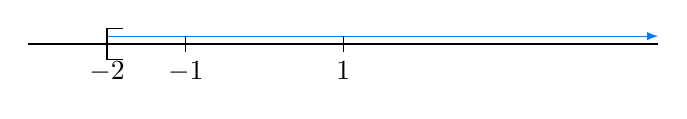
\begin{tikzpicture}
			\draw (-3,0) -- (5,0);
			\draw (-1.8,0.2) -- (-2,0.2) -- (-2,-0.2) -- (-1.8,-0.2);
			\draw[lightblue, -latex] (-2,0.1) -- (5,0.1);
			\foreach \x in {-2,-1,1}{\draw (\x,0.1) -- (\x,-0.1) node[below] {$\x$};}
		\end{tikzpicture}
	\end{center}
	$\bboxed{\dom(f\cdot g)=[-2,-1)\cup(-1,1)\cup(1,+\infty)}$
	
	$\left(\dfrac{f}{g}\right)(x)=\dfrac{f(x)}{g(x)}=\dfrac{\frac{1}{x^2}}{\sqrt{x+2}}=\dfrac{1}{(x^2-1)\sqrt{x+2}}\longrightarrow\bboxed{\left(\dfrac{f}{g}\right)(x)=\dfrac{1}{(x^2-1)\sqrt{x+2}}}$
	
	\begin{itemize}
		\item Por la raíz tenemos que $x+2\ge0\longrightarrow\bboxed{x\ge-2}$
		\item Por el cociente: \[ \begin{array}{l}
			x^2-1=0\longrightarrow x^2=1\longrightarrow \bboxed{x=\pm1}\text{ No puede ser}\\
			x+2=0\longrightarrow x=-2\longrightarrow\text{ No puede ser}
		\end{array} \]
	\end{itemize}
		\begin{center}
			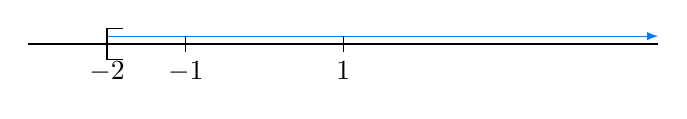
\begin{tikzpicture}
			\draw (-3,0) -- (5,0);
			\draw (-1.8,0.2) -- (-2,0.2) -- (-2,-0.2) -- (-1.8,-0.2);
			\draw[lightblue, -latex] (-2,0.1) -- (5,0.1);
			\foreach \x in {-2,-1,1}{\draw (\x,0.1) -- (\x,-0.1) node[below] {$\x$};}
		\end{tikzpicture}
		\end{center}
	$\bboxed{\dom\left(\dfrac{f}{g}\right)=[-2,-1)\cup(-1,1)\cup(1,+\infty)}$
\end{itemize}
\item \lb{Calcula los siguientes límites}

\begin{minipage}{0.6\textwidth}
	$\db{\lim_{x\to0}(\cos3x)^{\frac{1}{x^2}}=}(1^\infty)=e^{\displaystyle\lim_{x\to 0}\frac{1}{x^2}(\cos3x-1)}=e^{\displaystyle\lim_{x\to0}\frac{\cos3x-1}{x^2}}=\lb{(\ast)}$\\
	$\lb{(\ast)=}\lim_{x\to0}\dfrac{\cos3x-1}{x^2}=\left(\dfrac{0}{0}\right)=\left\{\begin{array}{l}
		\text{Equivalencias}\\
		\cos x\leadsto_01-\frac{x^2}{2}\\
		\cos(3x)\leadsto_01-\frac{(3x)^2}{2}
	\end{array}\right\}=\lim_{x\to0}\dfrac{\cancel{1}-\frac{9x^2}{2}-\cancel{1}}{x^2}=\lim_{x\to0}\dfrac{-\frac{9}{2}x^2}{x^2}=\bboxed{-\dfrac{9}{2}}$
\end{minipage}\qquad\begin{minipage}{0.3\textwidth}
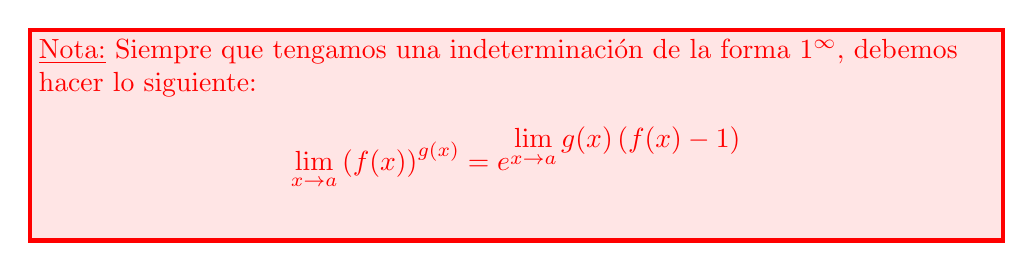
\begin{tikzpicture}
	\node[red, draw=red, fill=red!10, line width=1.5, text width=\linewidth] {\underline{Nota:} Siempre que tengamos una indeterminación de la forma $1^\infty$, debemos hacer lo siguiente: \[ \lim_{x\to a}\left(f(x)\right)^{g(x)}=e^{\displaystyle\lim_{x\to a}g(x)\left(f(x)-1\right)} \]};
\end{tikzpicture}
\end{minipage}
\item \lb{Analiza la continuidad de las siguientes funciones \[ f(x)=\begin{cases}
		x^2-4 & x<-2\\
		x+1 & -2\le x<2\\
		2x-1 & x\ge2
	\end{cases} \]}

$\forall x<-2\longrightarrow f(x)$ es continua\\
$\forall x\in(-2,2)\longrightarrow f(x)$ es continua\\
$\forall x\ge2\longrightarrow f(x)$ es continua\\
Veamos ahora si es continua en los puntos de cambio de trozo:
\begin{itemize}[label=]
	\item \underline{$x=-2$:}
	\begin{center}
		$\begin{rcases}
			\lim_{x\to-2^-}(x^2-4)=0\\
			\lim_{x\to-2^+}(x+1)=-1
		\end{rcases}~~\nexists\lim_{x\to-2}f(x)\longrightarrow $\begin{minipage}[t]{0.4\textwidth}
		$f(x)$ No es continua en $x=-2$, en concreto presenta una discontinuidad inevitable de salto finito.
		\end{minipage}
	\end{center}
	\item \underline{$x=2$}
	\begin{center}
		$\begin{rcases}
			\lim_{x\to2^-}(x+1)=3\\
			\lim_{x\to2^+}2x-1=3\\
			f(2)=3
		\end{rcases}~~f(x)$ es continua en $x=2$
	\end{center}
\end{itemize}
\fcolorbox{lightblue}{lightblue!10}{$f(x)$ es continua $\forall x\in\R-\{-2\}$}
\item \lb{Analiza la continuidad de las siguientes funciones \[ p(x)=\begin{cases}
		\frac{1}{x} & x<0\\
		x+1 & 0\le x\le 3\\
		\frac{1}{x^2-9} & x>3
	\end{cases} \]}

$\forall x<0\longrightarrow p(x)$ es continua.\\
$\forall x\in(0,3)\longrightarrow p(x)$ es continua.\\
$\forall x>3\longrightarrow p(x)$ es continua.\\
Nos falta comprobar si $p(x)$ es continua en $x=0$ y $x=3$.

\begin{itemize}[label=]
	\item \bboxed{x=0}
	\begin{center}
		$\begin{rcases}
			\lim_{x\to0^-}\dfrac{1}{x}=\dfrac{1}{0^-}=-\infty\\
			\lim_{x\to0^+}(x+1)=1
		\end{rcases}~~\nexists \lim_{x\to0}p(x)\longrightarrow~~$\begin{minipage}[t]{0.4\textwidth}
		$p(x)$ no es continua en $x=0$. En concreto tenemos diremos que presenta una discontinuidad inevitable de salto infinito. Habrá una asíntota vertical en $x=0$
		\end{minipage}
	\end{center}
	\item \bboxed{x=3}
	\begin{center}
		$\begin{rcases}
			\lim_{x\to3^-}(x+1)=4\\
			\lim_{x\to3^+}\dfrac{1}{x^2-9}=\dfrac{1}{0^+}=+\infty
		\end{rcases}~~\nexists \lim_{x\to3}p(x)\longrightarrow$\begin{minipage}[t]{0.4\textwidth}
		$p(x)$ no es continua en $x=3$. En concreto diremos que presenta una discontinuidad inevitable de salto infinito. Habrá una asíntota vertical en $x=3$.
		\end{minipage}
	\end{center}
\end{itemize}
\item \lb{Representa la función $y=x^2+4x+4$ e indica cuál es su recorrido.}

\begin{minipage}{0.45\textwidth}
	\begin{itemize}[leftmargin=*]
		\item Como el coeficiente líder es positivo: $\bigcup$
		\item Puntos de corte con el eje OX:
		\begin{center}
			$ x^2+4x+4\longrightarrow x=\dfrac{-4\pm\sqrt{16-16}}{2}\linebreak=\dfrac{-4\pm0}{2}=-2\text{ (doble)}\longrightarrow P(-2,0) $
		\end{center}
		\item El vértice: $x_V=\dfrac{-b}{2a}=\dfrac{-4}{2}=-2\longrightarrow \underset{y(-2)=0}{V(-2,0)}$
	\end{itemize}
	Cuando no tenemos puntos de corte con el eje OC o coincide con el vértice, entonces tomamos la imagen de dos puntos que estén a ambos lados del vértice y a la misma distancia:
\end{minipage}\qquad\begin{minipage}{0.45\textwidth}
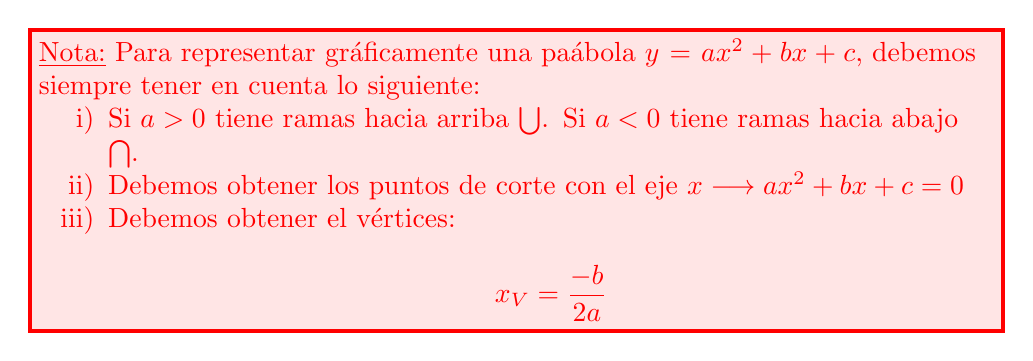
\begin{tikzpicture}
	\node[red, draw=red, fill=red!10, line width=1.5, text width=\linewidth] {\underline{Nota:} Para representar gráficamente una paábola $y=ax^2+bx+c$, debemos siempre tener en cuenta lo siguiente:
	
	\begin{enumerate}[label=\roman*)]
		\item Si $a>0$ tiene ramas hacia arriba $\bigcup$. Si $a<0$ tiene ramas hacia abajo $\bigcap$.
		\item Debemos obtener los puntos de corte con el eje $x\longrightarrow ax^2+bx+c=0$
		\item Debemos obtener el vértices:\[ x_V=\dfrac{-b}{2a} \]
		\end{enumerate}};
\end{tikzpicture}
\end{minipage}

\begin{itemize}[label=]
	\item $x=-3\longrightarrow y(-3)=9-12+4=1$
	\item $x=-1\longrightarrow y(-1)=1-4+4=1$
\end{itemize}
\begin{center}
	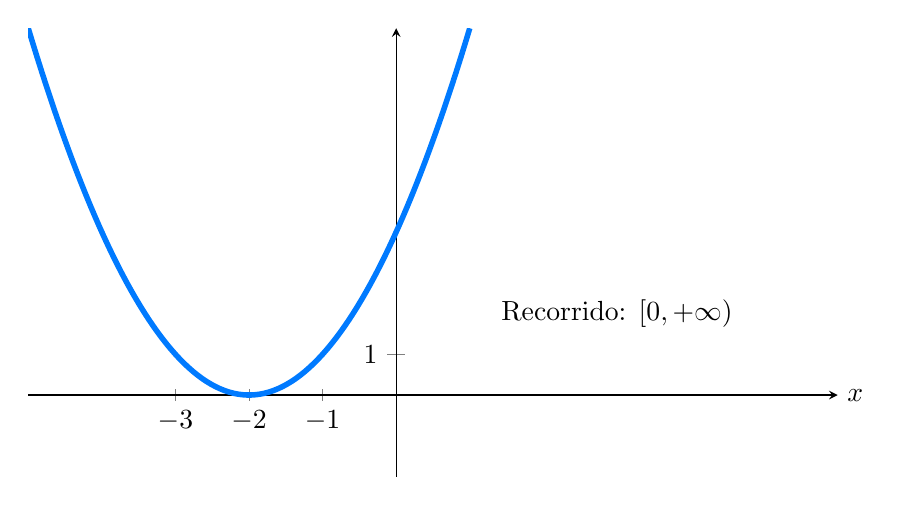
\begin{tikzpicture}
		\begin{axis}[
			xlabel={$x$},
			samples=100,
			axis lines=center,
			xtick={-3,-2,-1},
			ytick={1},
			xmax=6,
			ymin=-2,
			xscale=1.5,
			xlabel style={anchor=west},
			ylabel style={anchor=south},
			]
			\addplot[lightblue,domain=-5:1, line width=2] {x^2 + 4*x + 4};
			\node at (axis cs:3,2) {Recorrido: $[0,+\infty)$};
		\end{axis}
	\end{tikzpicture}
\end{center}
\item \lb{Representa la función $y=-x^2+2x+15$ e indica su recorrido.}
\begin{itemize}
	\item Como el coeficiente líder es negativo (-1) entonces la parabola es $\bigcap$.
	\item Puntos de corte con el eje OX: \[ -x^2+2x+15=0\longrightarrow x=\dfrac{-2\pm\sqrt{4+60}}{-2}=\dfrac{-2\pm8}{-2}\begin{cases}
		-3 & P(-3,0)\\
		5 & P(5,0)
	\end{cases} \]
	\item Vértice: $x_V=\dfrac{-b}{2a}=\dfrac{-2}{-2}=1\longrightarrow\begin{array}{l}
		x_V=1\\
		y(1)=-1+2+15=16
	\end{array}V=(1,16)$
\end{itemize}
\begin{center}
	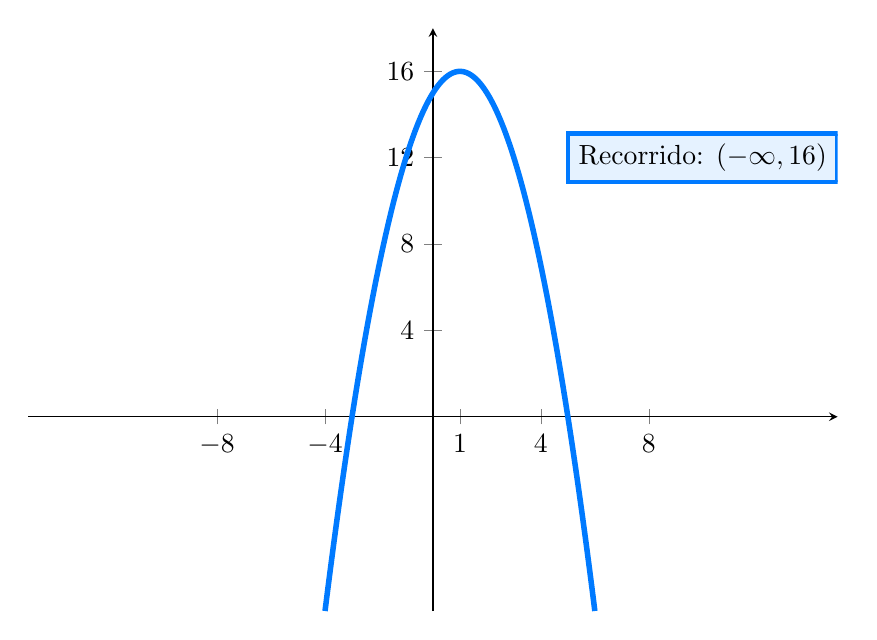
\begin{tikzpicture}
		\begin{axis}[
			axis lines=center,
			xmin=-15, xmax=15,
			xtick={-8,-4,1,4,8},
			ytick={0, 4, ..., 16},
			ymax=18, yscale=1.3,
			samples=1000,
			xscale=1.5,
			]
			\addplot[lightblue,domain=-4:6, line width=2] {-x^2+2*x+15};
			\node at (axis cs:10,12) {\fcolorbox{lightblue}{lightblue!10}{Recorrido: $(-\infty,16)$}};
		\end{axis}
	\end{tikzpicture}
\end{center}
\item \lb{Dadas las funciones $f(x)=x+3,\:g(x)=x+1$, calcula las funciones $g\circ f$ y $f\circ g$.}

Realizar una composición de funciones consiste en realizar una función, y justo donde termina esta empezaría la otra, tomando las imágenes de lo primero como los elementos de la segunda.

\begin{center}
\begin{minipage}{0.55\textwidth}
		\begin{tabular}{cll}
	$\bboxed{g\circ f}$ & \begin{tikzcd}[nodes={anchor=west}, row sep=tiny]
		\mathbb{R} \arrow[r, "f"] \arrow[rr, "g\circ f", bend left] & \mathbb{R} \arrow[r, "g"] & \mathbb{R}                \\
		x \arrow[r]                                                 & f(x) \arrow[r]            & g\left(f(x)\right)        \\
		x \arrow[r]                                                 & x+3 \arrow[r]             & (x+3)+1 \arrow[d, lightblue]         \\
		&                           & \lb{x+1} \arrow[lu, bend left, lightblue]
	\end{tikzcd} & $\bboxed{(g\circ f)(x)=x+4}$\\
	$\bboxed{f\circ g}$ & \begin{tikzcd}[nodes={anchor=west}, row sep=tiny]
		\mathbb{R} \arrow[r, "g"] \arrow[rr, "f\circ g", bend left] & \mathbb{R} \arrow[r, "f"] & \mathbb{R}         \\
		x \arrow[r]                                                 & f(x) \arrow[r]            & f\left(g(x)\right) \\
		x \arrow[r]                                                 & x+1 \arrow[r]             & (x+1)+3           
	\end{tikzcd}& $\bboxed{(f\circ g)(x)=x+4}$
\end{tabular}
\end{minipage}\qquad\begin{minipage}{0.25\textwidth}
\lb{Es Casualidad que salgan iguales. No tiene por qué.}
\end{minipage}
\end{center}
\item \lb{Dadas las funciones $f(x)=\dfrac{1}{x^2-1}$ y $g(x)=\sqrt{x+2}$. Con las funciones del ejercicio anterior, calcula $g\circ f$ y $f\circ g$.}
\begin{center}
	\begin{tabular}{lll}
	$\bboxed{g\circ f}$ & \begin{tikzcd}[nodes={anchor=west}, row sep=tiny]
		\mathbb{R} \arrow[r, "g"] \arrow[rr, "f\circ g", bend left] & \mathbb{R} \arrow[r, "f"] & \mathbb{R}         \\
		x \arrow[r]                                                 & f(x) \arrow[r]            & f\left(g(x)\right) \\
		x \arrow[r]                                                 & \dfrac{1}{x^2-1} \arrow[r]             & \sqrt{\dfrac{1}{x^2-1}+2}=\sqrt{\dfrac{2x^2-1}{x^2-1}}
	\end{tikzcd} & $\bboxed{\left(g\circ f\right)(x)=\sqrt{\dfrac{2x^2-1}{x^2-1}}}$\\
	$\bboxed{f\circ g}$ & \begin{tikzcd}[nodes={anchor=west}, row sep=tiny]
		\mathbb{R} \arrow[r, "g"] \arrow[rr, "f\circ g", bend left] & \mathbb{R} \arrow[r, "f"] & \mathbb{R}         \\
		x \arrow[r]                                                 & f(x) \arrow[r]            & f\left(g(x)\right) \\
		x \arrow[r]                                                 & \sqrt{x+2} \arrow[r]             & \dfrac{1}{(\sqrt{x+2})^2-1}=\dfrac{1}{x+1}
	\end{tikzcd} & $\bboxed{\left(f\circ g\right)(x)=\dfrac{1}{x+1}}$
\end{tabular}
\end{center}

\item \lb{Haz lo mismo con las funciones $f(x)=\sqrt{x+3},\:g(x)=\dfrac{x+1}{x+2}$, calcula las funciones $g\circ f$ y $f\circ g$.}

\begin{center}
	\begin{tabular}{lll}
		$\bboxed{g\circ f}$ & \begin{tikzcd}[nodes={anchor=west}, row sep=tiny]
			\mathbb{R} \arrow[r, "g"] \arrow[rr, "f\circ g", bend left] & \mathbb{R} \arrow[r, "f"] & \mathbb{R}         \\
			x \arrow[r]                                                 & f(x) \arrow[r]            & f\left(g(x)\right) \\
			x \arrow[r]                                                 & \sqrt{x+3} \arrow[r]             & \dfrac{\sqrt{x+3}+1}{\sqrt{x+3}+2}
		\end{tikzcd} & $\bboxed{\left(g\circ f\right)(x)=\dfrac{\sqrt{x+3}+1}{\sqrt{x+3}+2}}$\\
		$\bboxed{f\circ g}$ & \begin{tikzcd}[nodes={anchor=west}, row sep=tiny]
			\mathbb{R} \arrow[r, "g"] \arrow[rr, "f\circ g", bend left] & \mathbb{R} \arrow[r, "f"] & \mathbb{R}         \\
			x \arrow[r]                                                 & f(x) \arrow[r]            & f\left(g(x)\right) \\
			x \arrow[r]                                                 & \dfrac{x+1}{x+2} \arrow[r]             & \sqrt{\dfrac{x+1}{x+2}+3}=\sqrt{\dfrac{4x+7}{x+2}}
		\end{tikzcd} & $\bboxed{\left(f\circ g\right)(x)=\sqrt{\dfrac{4x+7}{x+2}}}$
	\end{tabular}
\end{center}

\item \lb{Calcula el dominio de las siguientes funciones: \[ y=\sqrt{\dfrac{x^2-4}{x^2+1}} \]}
\begin{itemize}
	\item Lo primero que tenemos es un cociente, por lo tanto, el denominador no puede ser cero. \[ x^2+1\neq0 \]
	\item Como tenemos una raíz cuadrada, entonces lo de dentro no puede ser negativo: \[ \dfrac{x^2-4}{x^2+1}=0 \]
\end{itemize}
\begin{center}
			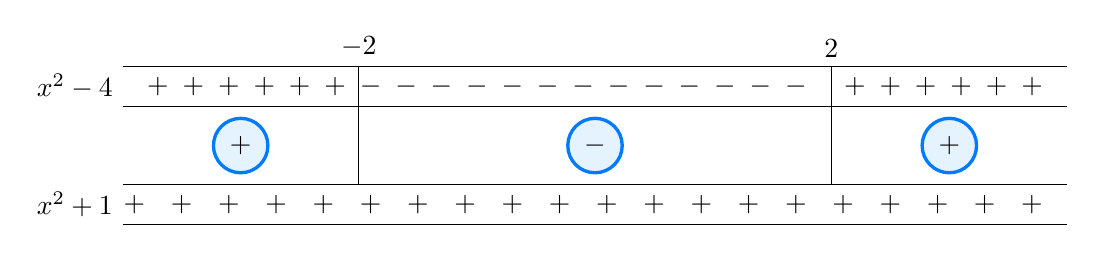
\begin{tikzpicture}[xscale=1.5]
		\draw (-4,0) -- (4,0)
		(-4,-0.5) -- (4,-0.5)
		(-4,-1.5) -- (4,-1.5)
		(-4,-2) -- (4,-2);
		\node[left] at (-4,-0.25-1.5) {$x^2+1$};
		\node[left] at (-4,-1.75+1.5) {$x^2-4$};
		\foreach \x in {-1.9, -1.6, ..., 1.9}{
			\node at (\x, -1.75+1.5) {$-$};
		}
		\foreach \x in {-3.9, -3.5, ..., 3.9}{
			\node at (\x, -0.25-1.5) {$+$};
		}
		\foreach \x in {2.2, 2.5, ..., 4}{
			\node at (\x, -1.75+1.5) {$+$};
		}
		\foreach \x in {-2.2, -2.5, ..., -4}{
			\node at (\x, -1.75+1.5) {$+$};
		}
		\draw (-2,0) node[above] {$-2$} -- (-2,-1.5)  ;
		\draw (2,0) node[above] {$2$} -- (2,-1.5)  ;
		\node[circle, draw=lightblue, line width=1.2, fill=lightblue!10] at (-3,-1) {+};
		\node[circle, draw=lightblue, line width=1.2, fill=lightblue!10] at (3,-1) {+};
		\node[circle, draw=lightblue, line width=1.2, fill=lightblue!10] at (0,-1) {$-$};
	\end{tikzpicture}
\end{center}
$\bboxed{\dom(f)=(-\infty,-2]\cup[2,+\infty)}$

\item \lb{Calcula el dominio de las siguientes funciones: \[ y=\sqrt{\dfrac{(x-1)(x-3)}{(x+2)(x-2)}} \]}

\begin{itemize}[leftmargin=*]
	\item Para empezar tenemos un cociente, y debe verificar que su denominador sea distinto de cero:
	\begin{itemize}[label=]
		\item $x+2=0\longrightarrow \bboxed{x=-2}$ No pertenece al $\dom(f)$
		\item $x-2=0\longrightarrow\bboxed{x=2}$ No pertenece al $\dom(f)$
	\end{itemize}
	\item Como tenemos una raíz cuadrada lo de dentro no puede ser negativo: \[ \dfrac{(x-1)(x-3)}{(x+2)(x-2)}\ge0 \]
\end{itemize}
\begin{center}
	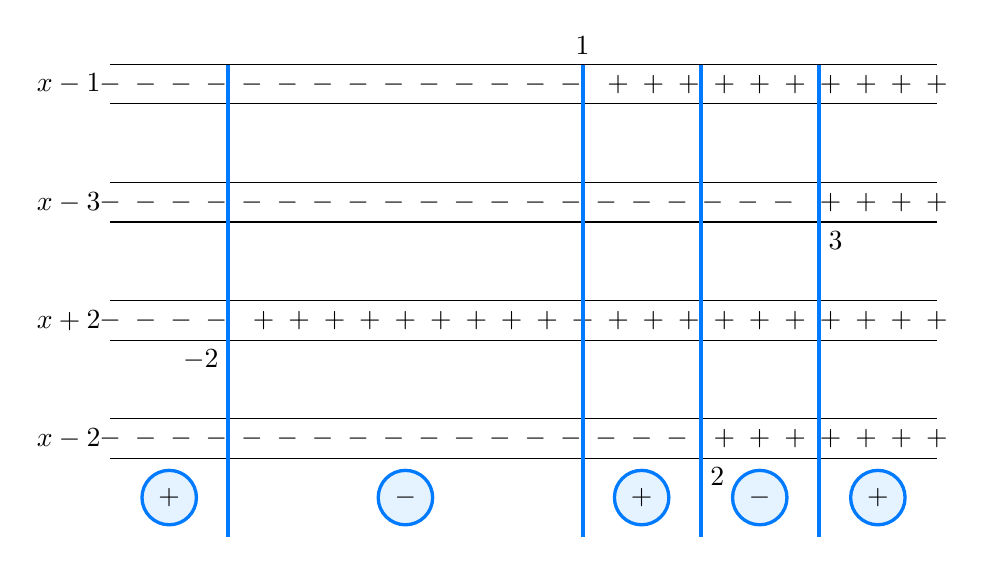
\begin{tikzpicture}[xscale=1.5]
		\foreach \y in {0,-0.5,-1.5,-2,-3,-3.5,-4.5,-5}{\draw (-3,\y) -- (4,\y);}
		\node[left] at (-3,-0.25) {$x-1$};
		\node[left] at (-3,-1.75) {$x-3$};
		\node[left] at (-3,-3.25) {$x+2$};
		\node[left] at (-3,-4.75) {$x-2$};
		\foreach \x in {-2.5,1.5,3.5}{\node[circle, draw=lightblue, line width=1.2, fill=lightblue!10] at (\x,-5.5) {+};}
		\foreach \x in {-0.5,2.5}{\node[circle, draw=lightblue, line width=1.2, fill=lightblue!10] at (\x,-5.5) {$-$};}
		\foreach \x in {-3, -2.7, ..., 1}{\node at (\x,-0.25) {$-$};}
		\foreach \x in {-3, -2.7, ..., 3}{\node at (\x,-1.75) {$-$};}
		\foreach \x in {-3, -2.7, ..., -2}{\node at (\x,-3.25) {$-$};}
		\foreach \x in {-3, -2.7, ..., 2}{\node at (\x,-4.75) {$-$};}
		\foreach \x in {4, 3.7, ..., 1}{\node at (\x,-0.25) {$+$};}
		\foreach \x in {4, 3.7, ..., 3}{\node at (\x,-1.75) {$+$};}
		\foreach \x in {4, 3.7, ..., -2}{\node at (\x,-3.25) {$+$};}
		\foreach \x in {4, 3.7, ..., 2}{\node at (\x,-4.75) {$+$};}
		\node[above] at (1,0) {$1$};
		\node[below right] at (3, -2) {$3$};
		\node[below left] at (-2, -3.5) {$-2$};
		\node[below right] at (2,-5) {$2$};
		\foreach \x in {-2,1,2,3}{\draw[lightblue, line width=1.5] (\x,0) -- (\x,-6);}
	\end{tikzpicture}
\end{center}
$\bboxed{\dom(f)=(-\infty,-2]\cup[1,2]\cup[3,+\infty)}$
\item \lb{Calcular \[ \lim_{x\to0^+}x^{\sin x} \]}
\begin{minipage}[b]{0.5\textwidth}
	$\lim_{x\to0^+}x^{\sin x}=(0^0)=\lim_{x\to0}e^{\log x^{\sin x}}=\lim_{x\to0}e^{\sin x\cdot\log x}=\lb{(\ast)}=e^0=\bboxed{1}$\\
	$\lb{(\ast)=}\lim_{x\to0}\sin x\cdot\log x=(0\cdot\infty)=\lim_{x\to0}\dfrac{\log x}{\frac{1}{\sin x}}=\left(\dfrac{\infty}{\infty}\right)=\left\{\text{L'Hôpital}\right\}=\lim_{x\to0}\dfrac{\frac{1}{x}}{\frac{-\cos x}{\sin^2 x}}=\lim_{x\to0}\dfrac{-\sin^2x}{x\cos x}=\left(\dfrac{0}{0}\right)=\left\{\begin{array}{l}
		\mathrm{Equivalencias}\\
		\sin x\leadsto_0 x
	\end{array}\right\}=\lim_{x\to0}\dfrac{-x^{\cancel{2}}}{\cancel{x}\cos x}=\lim_{x\to0}\dfrac{-x}{\cos x}=\dfrac{0}{1}=0$
\end{minipage}\qquad\begin{minipage}{0.4\textwidth}
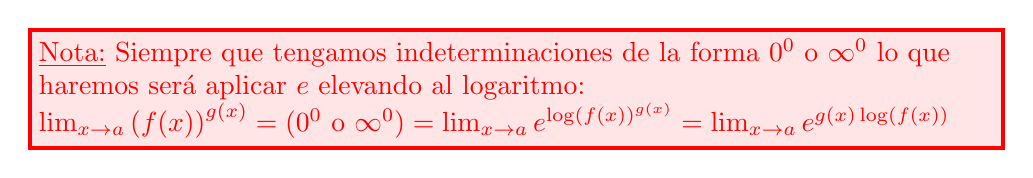
\begin{tikzpicture}
	\node[red, draw=red, fill=red!10, line width=1.5, text width=\linewidth] {\underline{Nota:} Siempre que tengamos indeterminaciones de la forma $0^0$ o $\infty^0$ lo que haremos será aplicar $e$ elevando al logaritmo: 
			
			$ \lim_{x\to a}\left(f(x)\right)^{g(x)}=(0^0\text{ o }\infty^0)=\lim_{x\to a}e^{\log\left(f(x)\right)^{g(x)}}=\lim_{x\to a}e^{g(x)\log\left(f(x)\right)} $};
\end{tikzpicture}\\
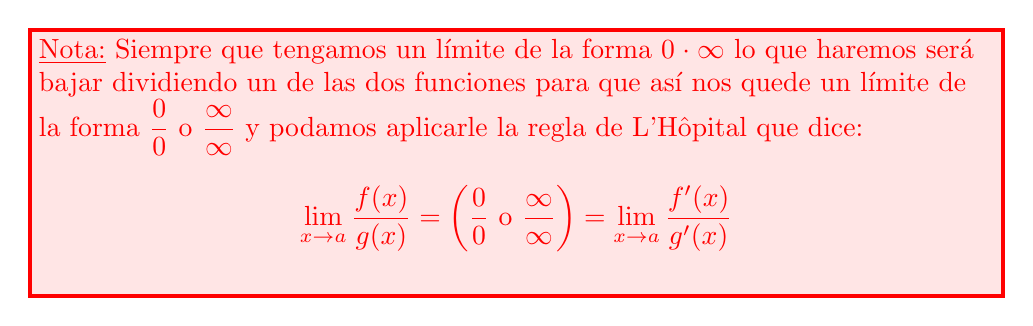
\begin{tikzpicture}
	\node[red, draw=red, fill=red!10, line width=1.5, text width=\linewidth] {\underline{Nota:} Siempre que tengamos un límite de la forma $0\cdot \infty$ lo que haremos será bajar dividiendo un de las dos funciones para que así nos quede un límite de la forma $\dfrac{0}{0}$ o $\dfrac{\infty}{\infty}$ y podamos aplicarle la regla de L'Hôpital que dice: \[ \lim_{x\to a}\dfrac{f(x)}{g(x)}=\left(\dfrac{0}{0}\text{ o }\dfrac{\infty}{\infty}\right)=\lim_{x\to a}\dfrac{f'(x)}{g'(x)} \]};
\end{tikzpicture}
\end{minipage}
\item \lb{Calcular \[ \lim_{x\to\frac{\pi}{2}^{-}}(\tan x)^{\cos x}. \]}

$\lim_{x\to\frac{\pi}{2}^{-}}(\tan x)^{\cos x}=(\infty^{0})=\lim_{ x \to \frac{\pi}{2}^{-} }e^{\log(\tan x)^{\cos x}}=\lim_{ x \to \frac{\pi}{2}^{-} }=\lb{(\ast)}=e^0=\bboxed{1}$

$\lb{(\ast)=}\lim_{ x \to \frac{\pi}{2}^{-} }\cos x\cdot \log(\tan x)=(0\cdot \infty)=\lim_{ x \to \frac{\pi}{2}^{-} }\dfrac{\log(\tan x)}{\frac{1}{\cos x}}=\left( \dfrac{\infty}{\infty} \right)=\left\{ \begin{array}{l}\text{Regla de}\\ \text{L'Hôpital}\end{array} \right\}=\lim_{ x \to \frac{\pi}{2}^{-} }\dfrac{\frac{1}{\tan x}\cdot \cancel{\frac{1}{\cos^{2}x}}}{\frac{\sin x}{\cancel{\cos^{2}x}}}=\linebreak\lim_{ x \to \frac{\pi}{2}^{-} }\frac{1}{\tan x\cdot \sin x}=\frac{1}{\infty}=0$

\item \lb{Calcular \[ \lim_{x\to1^+}\dfrac{x\sin(x-1)(1-\cos(x-1))}{(x-1)^3\ln(x-1)} \]}
$\lim_{x\to1^+}\dfrac{x\sin(x-1)(1-\cos(x-1))}{(x-1)^3\ln(x-1)}=\left(\dfrac{0}{0\cdot\infty}\right)=\lb{(\ast)}$

Podemos aplicar equivalencias:
\begin{itemize}[label=]
	\item $\sin x\leadsto_0x\longrightarrow\sin(x-1)\leadsto_0(x-1)$
	\item $\cos x\leadsto_01-\dfrac{x^2}{2}\longrightarrow1-\cos x\leadsto_0\dfrac{x^2}{2}\longrightarrow1-\cos(x-1)\leadsto_0\dfrac{(x-1)^2}{2}$
\end{itemize}
$\lb{(\ast)=}\lim_{x\to1^+}\dfrac{x\cdot\cancel{(x-1)}\cdot\frac{\cancel{(x-1)^2}}{2}}{\cancel{(x-1)^3}\cdot\ln(x-1)}=\lim_{x\to1^+}\dfrac{x}{2\ln(x-1)}=\dfrac{1}{-\infty}=\bboxed{0}$

\begin{center}
	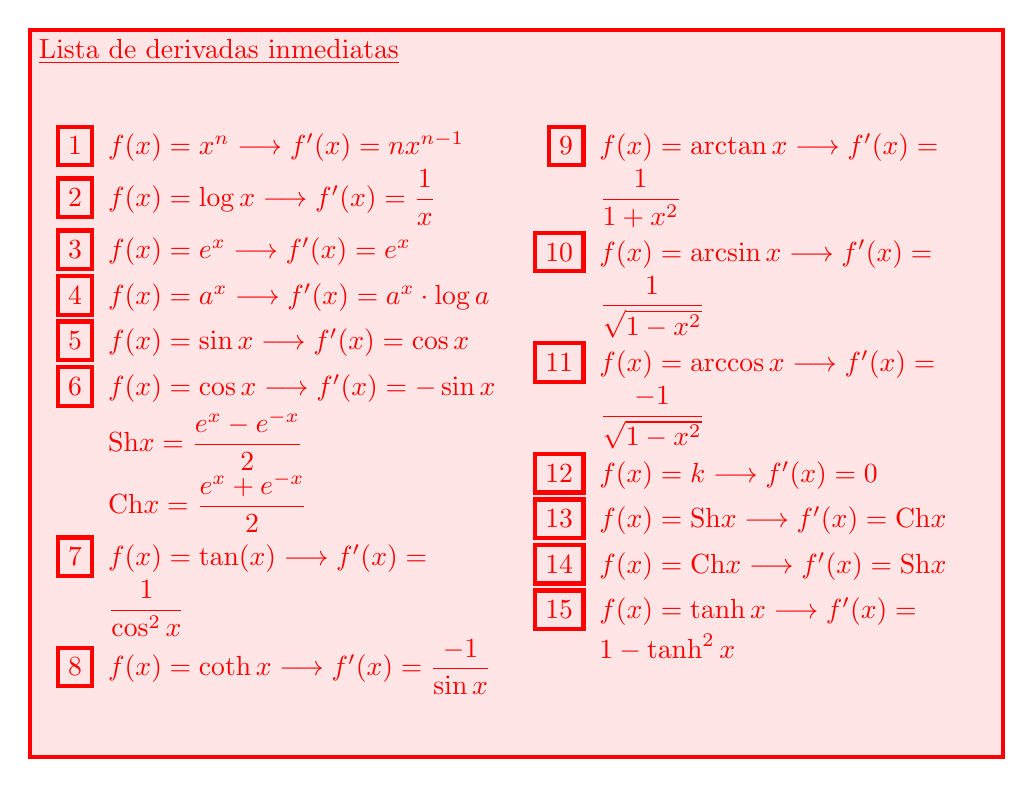
\begin{tikzpicture}
		\node[red, draw=red, fill=red!10, line width=1.5, text width=\linewidth] {
		\underline{Lista de derivadas inmediatas}
		\begin{multicols}{2}
			\begin{enumerate}[label=\boxed{\arabic*}]
			\item $f(x)=x^n\longrightarrow f'(x)=nx^{n-1}$
			\item $f(x)=\log x\longrightarrow f'(x)=\dfrac{1}{x}$
			\item $f(x)=e^{x}\longrightarrow f'(x)=e^{x}$
			\item $f(x)=a^x\longrightarrow f'(x)=a^x\cdot\log a$
			\item $f(x)=\sin x\longrightarrow f'(x)=\cos x$
			\item $f(x)=\cos x\longrightarrow f'(x)=-\sin x$
			
			$\mathrm{Sh}x=\dfrac{e^x-e^{-x}}{2}$
			
			$\mathrm{Ch}x=\dfrac{e^x+e^{-x}}{2}$
			\item $f(x)=\tan(x)\longrightarrow f'(x)=\dfrac{1}{\cos^2x}$
			\item $f(x)=\coth x\longrightarrow f'(x)=\dfrac{-1}{\sin x}$
			\item $f(x)=\arctan x\longrightarrow f'(x)=\dfrac{1}{1+x^2}$
			\item $f(x)=\arcsin x\longrightarrow f'(x)=\dfrac{1}{\sqrt{1-x^2}}$
			\item $f(x)=\arccos x\longrightarrow f'(x)=\dfrac{-1}{\sqrt{1-x^2}}$
			\item $f(x)=k\longrightarrow f'(x)=0$
			\item $f(x)=\mathrm{Sh}x\longrightarrow f'(x)=\mathrm{Ch}x$
			\item $f(x)=\mathrm{Ch}x\longrightarrow f'(x)=\mathrm{Sh}x$
			\item $f(x)=\tanh x\longrightarrow f'(x)=1-\tanh^2 x$
		\end{enumerate}
		\end{multicols}
		~~
		};
	\end{tikzpicture}
	
	\vspace{0.5cm}
	
	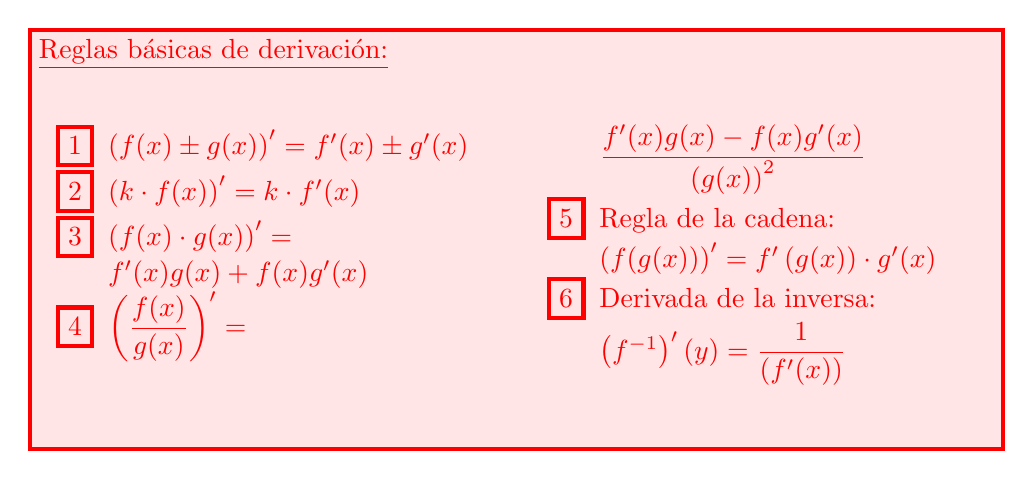
\begin{tikzpicture}
		\node[red, draw=red, fill=red!10, line width=1.5, text width=\linewidth] {\underline{Reglas básicas de derivación:}\\
		
		\begin{multicols}{2}
			\begin{enumerate}[label=\boxed{\arabic*}]
				\item $\left(f(x)\pm g(x)\right)'=f'(x)\pm g'(x)$
				\item $\left(k\cdot f(x)\right)'=k\cdot f'(x)$
				\item $\left(f(x)\cdot g(x)\right)'=f'(x)g(x)+f(x)g'(x)$
				\item $\left(\dfrac{f(x)}{g(x)}\right)'=\dfrac{f'(x)g(x)-f(x)g'(x)}{\left(g(x)\right)^2}$
				\item Regla de la cadena:
				
				$\left(f(g(x))\right)'=f'\left(g(x)\right)\cdot g'(x)$
				\item Derivada de la inversa:
				
				$\left(f^{-1}\right)'(y)=\dfrac{1}{\left(f'(x)\right)}$
			\end{enumerate}
		\end{multicols}
		~~
		};
	\end{tikzpicture}
\end{center}
\item \lb{Calcular las derivadas de las siguientes funciones:}
\begin{enumerate}[label=\color{red}\alph*)]
	\item $\db{f(x)=x^4+3x^2}\longrightarrow f'(x)=4x^2+6x$
	\item $\db{f(x)=x\sin x}$
	
	$f(x)=\lbb{x}{}\cdot\lbb{\sin x}{}$\\
	$f'(x)=1\cdot\sin x+x\cdot \cos x\longrightarrow\bboxed{f'(x)=\sin x+x\cos x}$
	\item $\db{f(x)=\dfrac{x}{2^x}}=x\cdot2^{-x}$
	
	$f'(x)=1\cdot 2^{-x}+x\cdot2^{-x}\cdot\log 2\cdot(-1)=2^{-x}\left[1-x\log2\right]\longrightarrow\bboxed{f'(x)=\dfrac{1-x\log2}{2^x}}$
\end{enumerate}
\item \lb{Calcular las derivadas de las siguientes funciones:}
\begin{enumerate}[label=\color{red}\alph*)]
	\item $\db{f(x)=\sqrt[3]{x^2+3x}}=(x^2+3x)^{\frac{1}{3}}$
	
	$f'(x)=\dfrac{1}{3}\left(x^2+3x\right)^{-\frac{2}{3}}\cdot(2x+3)=\dfrac{2x+3}{3\sqrt[3]{(x^2+3x)^2}}\longrightarrow\bboxed{f'(x)=\dfrac{2x+3}{3\sqrt[3]{(x^2+3x)^2}}}$
	\item $\db{f(x)=\sqrt{\cos x}}=(\cos x)^{\frac{1}{2}}$
	
	$f'(x)=\dfrac{1}{2}\left(\cos x\right)^{-\frac{1}{2}}\cdot(-\sin x)=\dfrac{-\sin x}{2\sqrt{\cos x}}\longrightarrow\bboxed{f'(x)=\dfrac{-\sin x}{2\sqrt{\cos x}}}$
	\item $\db{f(x)=\sin(x^3+3)}$
	
	$f'(x)=\cos(x^2+3)\cdot 2x\longrightarrow \bboxed{f'(x)=2x\cos(x^2+3)}$
\end{enumerate}
\item \lb{Calcular la derivada de las siguientes funciones:}
\begin{enumerate}[label=\color{red}\alph*)]
	\item $\db{f(x)=e^{x+\sin x}}\longrightarrow \bboxed{f'(x)=e^{x+\sin x}\cdot(1+\cos x)}$
	\item $\db{f(x)=\dfrac{\sin x}{x^2+5}}\longrightarrow \bboxed{f'(x)=\dfrac{\cos x\cdot(x^2+5)-2x\cdot\sin x}{(x^2+5)^2}}$
	\item $\db{f(x)=\ln\left(\dfrac{1+x}{1-x}\right)}$
	
	$f'(x)=\dfrac{1}{\left(\frac{1+x}{\cancel{1-x}}\right)}\cdot\dfrac{1\cdot(1-\cancel{x})+(1+\cancel{x})\cdot1}{(1-x)^{\cancel{2}}}=\dfrac{2}{(1+x)(1-x)}=\bboxed{\dfrac{2}{1-x^2}}$
\end{enumerate}
\item \lb{Calcular la derivada de las siguientes funciones:}
\begin{enumerate}[label=\color{red}\alph*)]
	\item $\db{f(x)=\arcsin\left(\ln x\right)}$
	
	$f'(x)=\dfrac{1}{\sqrt{1-(\ln x)^2}}\cdot\dfrac{1}{x}\longrightarrow\bboxed{f'(x)=\dfrac{1}{x\sqrt{1-(\ln x)^2}}}$
	\item $\db{f(x)=\sin(\arctan x)}$
	
	$f'(x)=\cos\left(\arctan x\right)\cdot\dfrac{1}{1+x^2}\longrightarrow\bboxed{f'(x)=\dfrac{\cos\left(\arctan x\right)}{1+x^2}}$
	
	\item $\db{f(x)=\cos\left(\dfrac{x}{e^x}\right)}=\cos(x\cdot e^{-x})$
	
	$f'(x)=-\sin(xe^{-x})\cdot\left[1\cdot e^{-x}+x\cdot e^{-x}\cdot(-1)\right]=\bboxed{-e^{-x}\sin(xe^{-x})[1-x]}$
\end{enumerate}
\item \lb{Calcular la derivada de la función inversa de $y=\sin x$.}

$\begin{array}{ll}
	\text{Tenemos }&f(x)=\sin x\longrightarrow f^{-1}(x)=\arcsin x\\
	&y=\sin x\xrightarrow{\qquad~} x=\arcsin y
\end{array}$

$\begin{array}{l}
	\left(f^{-1}(x)\right)'=\dfrac{1}{f'(x)}=\dfrac{1}{\cos(x)}=\dfrac{1}{\sqrt{1-y^2}}\longrightarrow\bboxed{\left(f^{-1}\right)'(y)=\dfrac{1}{\sqrt{1-y^2}}}\\
	\sin^2x+\cos^2x=1\longrightarrow\cos^2x=1-\sin^2x\longrightarrow\cos x=\sqrt{1-\sin^2x}=\left\{y=\sin x\right\}=\sqrt{1-y^2}
\end{array}$
\item \lb{Calcula los siguientes límites: \[ \lim_{x\to\infty}\dfrac{5x-4x^2-1}{2x^3-x-1} \]}
\begin{minipage}[b]{0.5\textwidth}
	$\lim_{x\to+\infty}\dfrac{-4x^2+5x-1}{2x^3-x-1}=\left(\dfrac{\infty}{\infty}\right)=\lim_{x\to+\infty}\dfrac{-\frac{4x^2}{x^3}+\frac{5x}{x^3}-\frac{1}{x^3}}{\frac{2x^3}{x^3}-\frac{x}{x^3}-\frac{1}{x^3}}=\lim_{x\to+\infty}\dfrac{\tozero{-\frac{4}{x}}+\tozero{\frac{5}{x^2}}-\tozero{\frac{1}{x^3}}}{2-\tozero{\frac{1}{x^2}}-\tozero{\frac{1}{x^3}}}=\dfrac{0}{2}=\bboxed{0}$
\end{minipage}\qquad\begin{minipage}{0.4\textwidth}
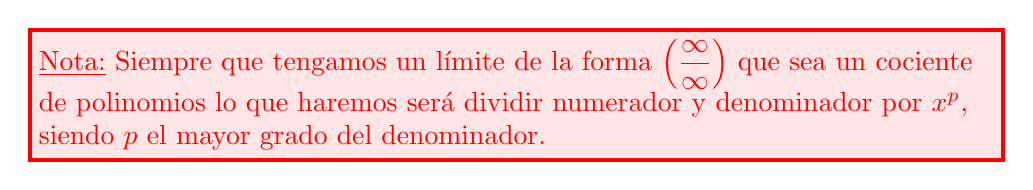
\begin{tikzpicture}
	\node[red, draw=red, fill=red!10, line width=1.5, text width=\linewidth] {\underline{Nota:} Siempre que tengamos un límite de la forma $\left(\dfrac{\infty}{\infty}\right)$ que sea un cociente de polinomios lo que haremos será dividir numerador y denominador por $x^p$, siendo $p$ el mayor grado del denominador.};
\end{tikzpicture}
\end{minipage}
\item \lb{Calcula los siguientes límites: \[ \lim_{x\to0}\dfrac{1-\cos3x}{x(x-2)\tan2x} \]}

$\lim_{ x \to 0 } \frac{1-\cos 3x}{x\lbb{(x-2)}{\begin{subarray}{c}
			\text{No da}\\
			\text{problemas}
	\end{subarray}}\tan(2x)}=\lim_{ x \to 0 } \dfrac{\frac{9x^{2}}{2}}{x(x-2)\cdot 2x}=\lim_{ x \to 0 }\dfrac{9\cancel{x^{2}}}{4\cancel{x^{2}}(x-2)}=\bboxed{-\frac{9}{8}}$

Equivalencias:

$\cos x\leadsto_{0}1-\cos x\leadsto_{0}\dfrac{x^{2}}{2}\longrightarrow 1-\cos (3x)\leadsto_{0}\dfrac{(3x)^2}{2}=\dfrac{9x^{2}}{2}$

$\tan x\leadsto_{0}x\longrightarrow\tan(2x)\leadsto_{0}2x$
\item \lb{Calcula los siguientes límites: \[ \lim_{x\to1}\dfrac{\log x}{x-\sqrt{x}} \]}

\begin{enumerate}[label=\underline{\arabic*ª Forma:}, leftmargin=2cm]
	\item ~~
	
	$\lim_{x\to1}\dfrac{\log x}{x-\sqrt{x}}=\left(\dfrac{0}{0}\right)=\left\{\text{Regla de L'Hôpital}\right\}=\lim_{x\to1}\dfrac{\frac{1}{x}}{1-\frac{1}{2\sqrt{x}}}=\dfrac{1}{1-\frac{1}{2}}=\bboxed{2}$
	\item ~~
	
	$\lim_{x\to1}\dfrac{\log x}{x-\sqrt{x}}=\left(\dfrac{0}{0}\right)=\lim_{x\to1}\dfrac{\log x\cdot(x+\sqrt{x})}{(x-\sqrt{x})(x+\sqrt{x})}=\lim_{x\to1}\dfrac{\log x\cdot(x+\sqrt{x})}{x^2-x}=\lim_{x\to1}\dfrac{\log x\cdot(x+\sqrt{x})}{x(x-1)}=\left(\dfrac{0}{0}\right)=\lim_{x\to1}\dfrac{\cancel{(x-1)}(x+\sqrt{x})}{x\cancel{(x-1)}}=\dfrac{2}{1}=\bboxed{2}$
\end{enumerate}
Equivalencias:

$\begin{array}{l}
	\log(1+x)\leadsto_{0}x\\
	\log(x)=\log\left(1+\bboxed{(x-1)}\right)\leadsto_1\bboxed{(x-1)}
\end{array}$
\end{enumerate}
\end{document}